\chapter{Wyniki}

\section{Wprowadzenie}

Dla wszystkich zaimplementowanych w poprzednim rozdziale algorytmów przeprowadzono testy pokazujące skuteczność ich działania na wybranych klasach grafów. Na początku przeprowadzono testy dla różnych kombinacji hiperparametrów algorytmu mrówkowego, w celu uzyskania najlepszego zestawu parametrów dla tego problemu, który będzie następnie wykorzystywany w dalszych rozważaniach. Następnie przedstawiono wyniki dla wybranych klas grafów:
\begin{itemize}
    \item grafy rzadkie
    \item grafy gęste
    \item drzewa
    \item grafy bezskalowe,
\end{itemize}
Grafy każdej klasy wygenerowano z następującą liczbą wierzchołków: ${10, 20, 30, 40, 50}$, dla każdej liczby wierzchołków po 3 razy. Dla spójności, wszystkie algorytmy, tam gdzie to ma sens, testowano na tych samych wygenerowanych grafach. Dalej w tabelach zostaną przedstawione wyniki poglądowe jednego z trzech takich zestawów. 
Wszystkie średnie pomiary czasów w tabelach przedstawiono w sekundach. Pomiary dla każdego przypadku wykonywano pięciokrotnie w celu otrzymania wiarygodnego wyniku. Pomiary mierzono w nanosekundach z niepewnością pomiaru wynoszącą 100 nanosekund, wykorzystując funkcję \textit{time.perf\_counter\_ns()}. Dodatkowo dla każdej klasy przedstawiono rysunki grafów z WCRDF po użyciu algorytmów oraz wykres porównujący czas działania każdego z algorytmów w zależności od liczby wierzchołków, w skali logarytmicznej.\\
W późniejszej części rozdziału rozważano również skuteczność algorytmów wyznaczających prawidłowe WCRDF, ale niekoniecznie optymalne $\gamma^{\text{wc}}_R(G)$.\\
Na podstawie wyników zostaną przedstawione obserwacje oraz wnioski dla każdej z klasy grafów oraz dla algorytmów niedokładnie wyznaczających $\gamma^{\text{wc}}_R(G)$.

\section{Hiperparametry algorytmu mrówkowego}

W algorytmie mrówkowym zostały zdefiniowane następujące parametry:
\begin{itemize}
    \item \textbf{\alpha} - wpływ poziomu feromonów na decyzję wyboru ścieżki. Przyjęte do testów wartości \\
    $\alpha = [3,1]$
    \item \textbf{\beta} - wpływ heurystyki lokalnej (liczby sąsiadów) na decyzję wyboru ścieżki. Przyjęte do testów wartości $\beta = [5,20]$
    \item \textbf{\rho} - współczynnik parowania feromonów, określający, jak szybko feromony zanikają. Przyjęte do testów wartości $\rho = [0.5, 0.7]$
    \item liczba mrówek w każdej iteracji. Przyjęte do testów wartości $[100,150]$
\end{itemize}

W poniższej tabeli zostały przedstawione, wybrane zestawy tych hiperparametrów osiągające najmniejszy średni błąd. Średni błąd był wyznaczany na podstawie dokładnego wyniku osiąganego przez algorytmy dokładnie wyznaczające $\gamma^{\text{wc}}_R(G)$ dla danego przykładu grafu.\\

\begin{table}[H]
    \centering
    \begin{tabular}{|c|c|c|c|c|}
        \hline
     \alpha & \beta & \rho & liczba mrówek & średni błąd \\  \hline
    3 & 20 & 0.5 & 150 & 7.933333 \\    \hline
    3 & 20 & 0.7 & 150 & 8.000000 \\    \hline
    1 & 5 & 0.7 & 150 & 8.000000 \\    \hline
    1 & 20 & 0.7 & 150 & 8.066667 \\    \hline
    1 & 20 & 0.5 & 100 & 8.066667 \\    \hline
\end{tabular}    
\caption{Wpływ kombinacji hiperparametrów na błąd rozwiązania}
\end{table}

Średni błąd wygląda na znaczny, ale można zauważyć, że ogólnie algorytm jest stabilny oraz kombinacja hiperparametrów nieznacznie wpływa na jakość osiąganych wyników.\\
Dominacja wartości $\beta = 20$ wskazuje na, to że algorytm bardziej polega na heurystyce lokalnej, którą jest liczba sąsiadów wierzchołka, w kontekście rozwiązania tego problemu, co jest spodziewanym wynikiem.\\
Dodatkowo, wolniejsze parowanie feromonów (\rho) zdaje się sprzyjać lepszym wynikom. Oznacza to, że dłuższe zapamiętywanie informacji o dobrych rozwiązaniach wpływa korzystnie na wynik.\\

Kolejna tabela przedstawia zestaw parametrów z najmniejszym średnim błędem dla danej klasy grafu.

\begin{table}[H]
    \centering
    \begin{tabular}{|c|c|c|c|c|c|}
        \hline
    Klasa grafów & \alpha & \beta & \rho & liczba mrówek & średni błąd \\     \hline
    ErdosRenyi\_dense & 1 & 20 & 0.5 & 100 & 6.5 \\     \hline
    ErdosRenyi\_sparse & 3 & 20 & 0.5 & 150 & 8.666667 \\     \hline
    RandomTree & 1 & 5 & 0.7 & 150 & 7.5 \\    \hline
    ScaleFree & 3 & 20 & 0.7 & 150 & 7.25 \\ \hline
\end{tabular}
\caption{Wpływ kombinacji hiperparametrów na błąd rozwiązania na konkretnych klasach grafów}
\end{table}

Dla grafów gęstych udało się dobrać korzystny zestaw hiperparametrów, dający stosunkowo niski średni błąd. W tym przypadku algorytm woli bardziej się skupić na heurystyce lokalnej niż na wpływie feromonów, co jest spodziewanym zachowaniem ze względu na to, że w grafach gęstych bardzo często dla WCRDF to wierzchołki o największym stopniu są najbardziej promowane.

Dla grafów rzadkich widoczny jest dodatkowo większy wpływ feromonów. Ze względu na rzadszą strukturę grafu, korzystnym zachowaniem jest zapamiętanie dobrego rozwiązania, a następnie eksploatowanie go. Podobnie dla grafów bezskalowych, jednakże kładziony jest tutaj nacisk na większą eksplorację, ze względu na to, że struktura grafu jest podobna do grafów rzadkich.

Drzewa w stosunku do pozostałych klas grafu mają najbardziej specyficzną strukturę i w tych wynikach się to również odzwierciedla. W tym przypadku nie jest kładziony nacisk na heurystykę lokalną, ponieważ w drzewach bardzo często wierzchołki o wysokich stopniach niekoniecznie należą do zbioru dominującego. Algorytm w tym przypadku jest bardziej nastawiony na eksplorację, bo można zaobserwować zrównoważony wpływ heurystyki lokalnej i feromonu, przy dużym współczynniku parowania.

Na podstawie powyższych parametrów można stwierdzić, że są one adekwatne do właściwości konkretnej struktury klasy grafu. Mimo to, średni błąd we wszystkich przypadkach jest znaczny, ale dosyć stabilny, nie ma wielkich różnic między klasami grafów.\\

Po tej analizie dokonano wyboru hiperparametrów, które będą użyte w dalszych rozważaniach. Został wybrany jeden zestaw ze względu na stabilność wartości średniego błędu między różnymi zestawami hiperparametrów, jak i między klasami grafów. Hiperparametry te zostały przedstawione w poniższej tabeli.

\begin{table}[H]
    \centering
    \begin{tabular}{|c|c|c|c|}
        \hline
     \alpha & \beta & \rho & liczba mrówek \\  \hline
    3 & 20 & 0.5 & 150  \\    \hline
\end{tabular}    
\caption{Wybrany zestaw parametrów}
\end{table}

Wybór ten oznacza, że heurystyka lokalna w postaci stopnia wierzchołka grafu oraz feromony będą miały istotny wpływ na wyniki algorytmu. Algorytm będzie zapamiętywał dobre wyniki i je eksploatował.

\section{Wyniki działania algorytmów}

Wybrane wyniki działania algorytmów zostały przedstawione w tabelach. Wyniki podzielono na sekcje względem liczby wierzchołków oraz posortowano według rosnącego czasu działania w obrębie każdej z sekcji.  Algorytmy ILP, ILP2, Brute Force oraz TreeLinear dla drzew są w tych przypadkach algorytmami optymalnie wyznaczającymi wartość $\gamma^{\text{wc}}_R(G)$ i to one stanowią wartość odniesienia dla dokładności pozostałych algorytmów.\\

Dodatkowo zostaną zaprezentowane wykresy przedstawiające średni czas działania każdego z algorytmów w stosunku do liczby wierzchołków w skali logarytmicznej. Wyniki zostały połączone liniami w celu lepszej wizualizacji i odzwierciedlenia tendencji wzrostu.\\

Następnie przedstawiono grafiki ukazujące WCRDF znalezione przez algorytmy dla przykładowego, 20-wierzchołkowego grafu analizowanej klasy, gdzie wartości 0 to żółte wierzchołki, 1 - niebieskie, a 2 to czerwone.

\subsection{Grafy rzadkie}

Grafy rzadkie charakteryzują się znacznie mniejszą liczbą krawędzi niż maksymalna możliwa, czyli $|E| \ll \frac{n(n - 1)}{2}$ oraz posiada przede wszystkim wierzchołki o niskim stopniu. Z racji mniejszej liczby krawędzi algorytmy programowania liniowego mogą sobie dobrze radzić, ze względu na mniejszą liczbę ograniczeń i zmiennych. Ze względu na nieregularną strukturę i komponenty o różnym stopniu połączenia, algorytmy deterministyczne mogą znacząco odbiegać od optymalnego wyniku.

\begin{table}[H]
    \centering
    \begin{tabular}{|c|c|c|c|c|}
    \hline
    Algorytm & Liczba wierzchołków & Liczba krawędzi & $\gamma^{\text{wc}}_R(G)$ & Średni czas (s) \\
    \hline
    Greedy	   & 10 &	15 &	5	 &   0,0000253	\\		
    ILP	       & 10 &	15 &	5	  &   0,03225824 \\
    ILP2	   & 10 &	15 &	5	  &   0,06530336 \\
    Approx	   & 10 &	15 &	6	  &   0,0716367 \\
    Brute Force & 10 &	15 &	5 	 &   1,22720146 \\
    AntColony & 10 &	15 &	5 	 &   1,9432132 \\
    \hline
    Greedy     &  20 & 61 & 7    &  0,00009044 \\     
    ILP        &  20 & 61 & 7    &   0,17597988 \\
    Approx     &  20 & 61 & 8    &    0,81655686 \\   
    ILP2       &  20 & 61 & 7    &   1,28852564 \\    
    AntColony  &  20 & 61 & 11   &   4,302339 \\         
    \hline
    Greedy & 30 & 122 & 10 & 0,00018332 \\
    ILP & 30 & 122 & 9 & 0,4925489 \\
    Approx & 30 & 122 & 10 & 1,27100858 \\
    ILP2 & 30 & 122 & 9 & 3,89847968 \\
    AntColony & 30 & 122 & 19 & 10,9692404 \\
    \hline
    Greedy & 40 & 215 & 11 & 0,00015998 \\
    ILP & 40 & 215 & 8 & 0,4383133 \\
    Approx & 40 & 215 & 10 & 3,70053236 \\
    ILP2 & 40 & 215 & 8 & 6,50026534 \\
    AntColony & 40 & 215 & 25 & 12,11287052 \\
    \hline
    Greedy & 50 & 353 & 10 & 0,00027048 \\
    ILP & 50 & 353 & 8 & 3,9218204 \\
    Approx & 50 & 353 & 10 & 4,86207684 \\
    AntColony & 50 & 353 & 30 & 28,00923878 \\
    ILP2 & 50 & 353 & 8 & 88,8271173 \\   
    \hline
    \end{tabular}
    \caption{Wyniki dla grafów rzadkich}
    \end{table}

    Analizując powyższe wyniki można zauważyć, że algorytm zachłanny Greedy charakteryzuje się bardzo szybkim czasem działania, a jakość rozwiązania jest bliska optymalnej.

    Algorytm mrówkowy wraz ze wzrostem liczby wierzchołków zaczyna dawać coraz gorsze wyniki, mimo wyboru dobrego dla tej klasy zestawu parametrów. Warto zaznaczyć również, że jest jednym z wolniej działających algorytmów.

    Wynik dla algorytmu Brute Force można zaobserwować wyłącznie dla 10 wierzchołków. Dzieje się tak, ponieważ zgodnie z pierwotnymi założeniami, już dla kilkunastu wierzchołków w dowolnym grafie, algorytm ten przestał zwracać wyniki w rozsądnym czasie.

    \begin{figure}[H]
        \centering
        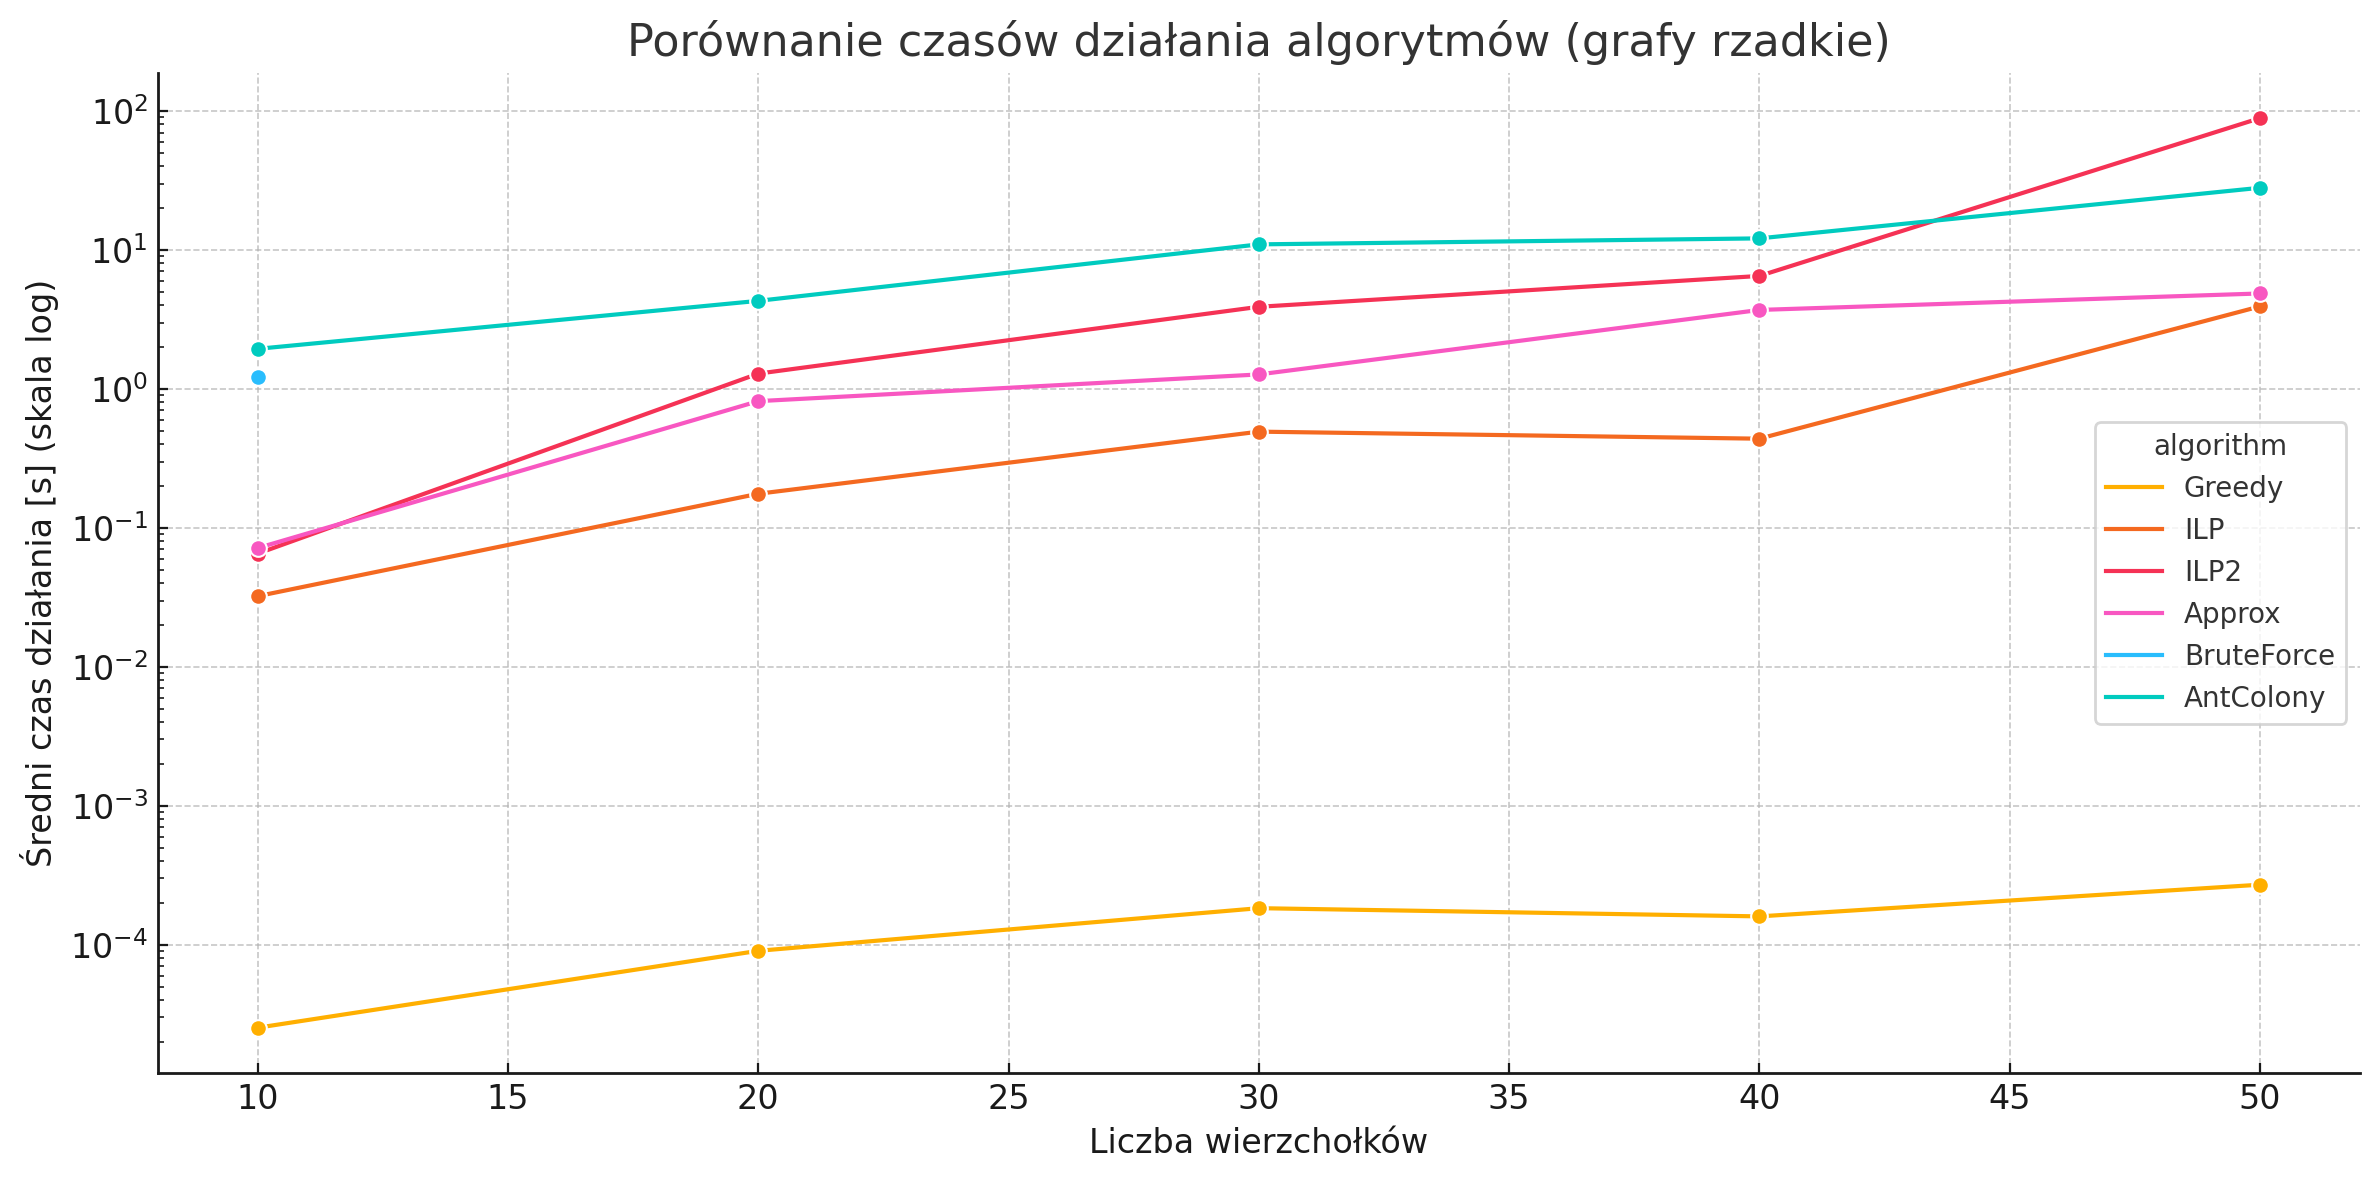
\includegraphics[width=\textwidth]{assets/sparse.png}
        \caption{Porównanie średniego czasu działania algorytmów na grafach rzadkich w stosunku do liczby wierzchołków w grafie.}
        \label{fig:sparsePlot}
    \end{figure}

    W tym przypadku znacznie wyróżnia się algorytm Greedy, który działa ponad 1000 razy szybciej niż pozostałe algorytmy, przy czym nie osiąga wyników znacznie odbiegających od optymalnego. Algorytmy ILP i ILP2 dają optymalny wynik, w rozsądnym czasie działania, przy czym ILP jest szybszy.

    Naturalnie, wraz ze wzrostem liczby wierzchołków, a co za tym idzie i krawędzi, czas pracy wszystkich algorytmów wydłuża się. Dla algorytmu zachłannego są to jednak na tyle krótkie czasy, że można stwierdzić, że algorytm będzie skalowalny i również wykonywalny w rozsądnym czasie dla większych grafów. Pozostałe algorytmy notują znaczny skok w czasie działania, zwłaszcza dla większej liczby wierzchołków.

    \begin{figure}[H]
        \centering
        \begin{subcaptionbox}*{}[0.48\linewidth]
            {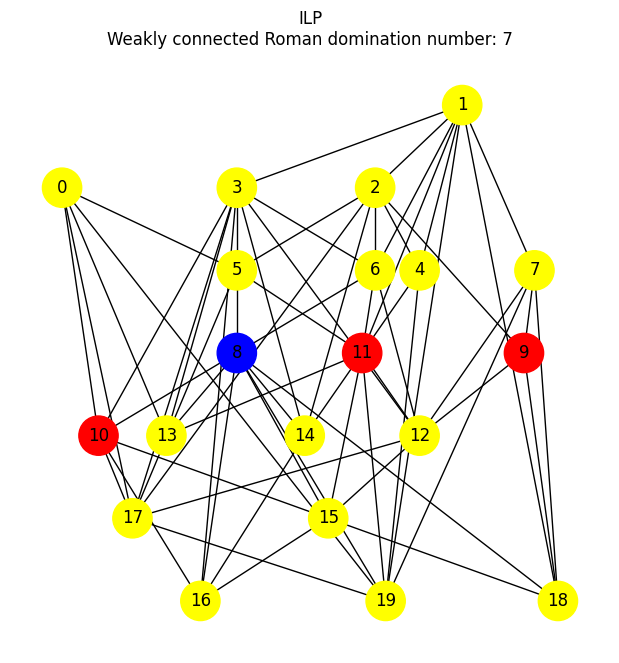
\includegraphics[width=0.75\linewidth]{assets/plots/ILP/ErdosRenyi_sparse_n20_i2_results.png}}
        \end{subcaptionbox}
        \hfill
        \begin{subcaptionbox}*{}[0.48\linewidth]
            {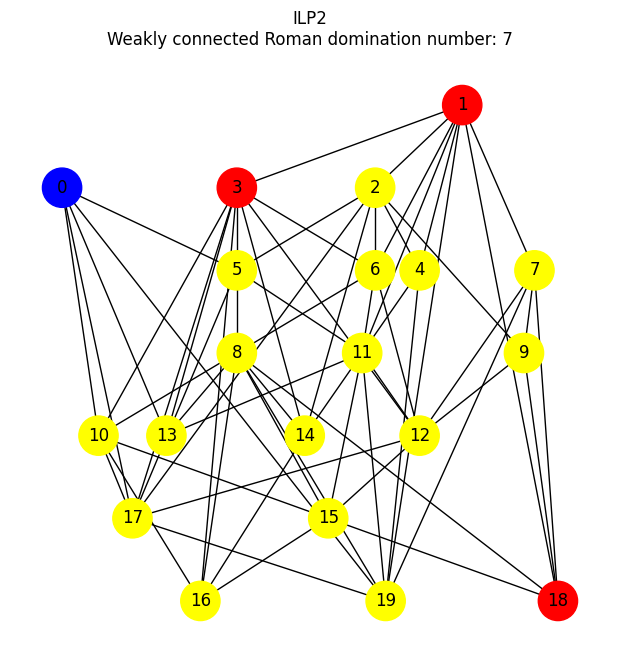
\includegraphics[width=0.75\linewidth]{assets/plots/ILP2/ErdosRenyi_sparse_n20_i2_results.png}}
        \end{subcaptionbox}
        \hfill
        \begin{subcaptionbox}*{}[0.48\linewidth]
            {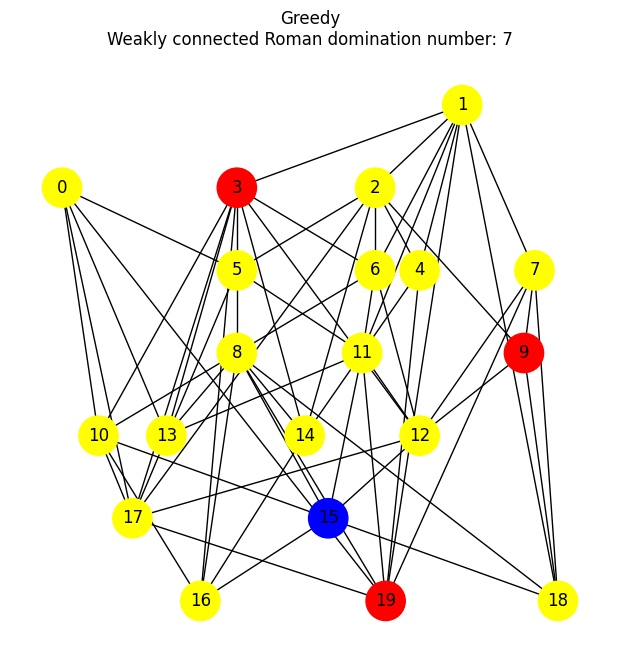
\includegraphics[width=0.75\linewidth]{assets/plots/Greedy/ErdosRenyi_sparse_n20_i2_results.png}}
        \end{subcaptionbox}
        \hfill
        \begin{subcaptionbox}*{}[0.48\linewidth]
            {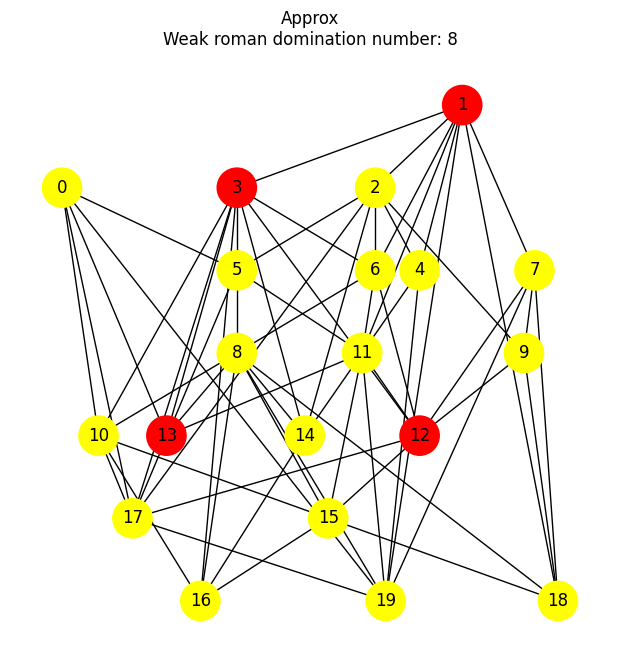
\includegraphics[width=0.75\linewidth]{assets/plots/Approx/ErdosRenyi_sparse_n20_i2_results.png}}
        \end{subcaptionbox}
        \hfill
        \begin{subcaptionbox}*{}[0.48\linewidth]
            {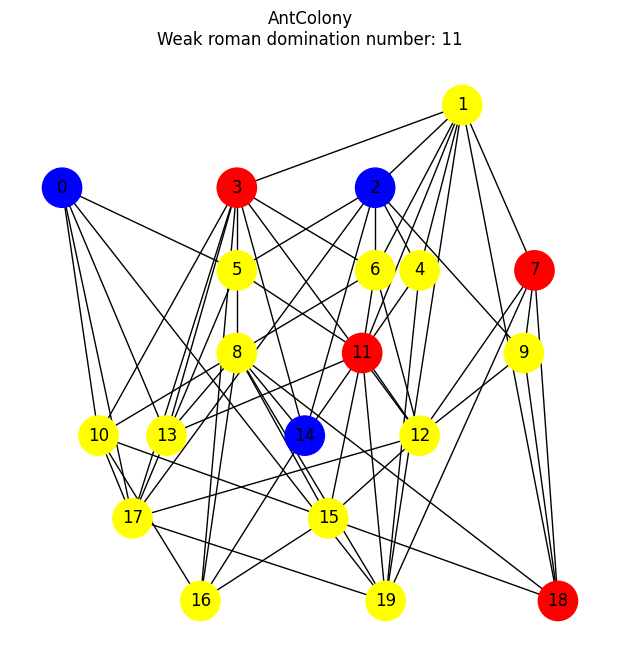
\includegraphics[width=0.75\linewidth]{assets/plots/AntColony/ErdosRenyi_sparse_n20_i2_results.png}}
        \end{subcaptionbox}
    
        \caption{Wyniki dla przykładowego grafu rzadkiego.}
        \label{fig:sparse}
    \end{figure}

\subsection{Grafy gęste}

Grafy gęste charakteryzują się dużą liczbą krawędzi, bliską $|E| \leq \frac{n(n - 1)}{2}$. Wierzchołki mają duże stopnie i dominowanie jednego wierzchołka pokrywa znaczną część grafu. Dlatego algorytmy przybliżone powinny łatwo i szybko znajdować dobre rozwiązania. Z racji dużej liczby zmiennych i ograniczeń algorytmy ILP/ILP2 powinny charakteryzować się dłuższym czasem działania.

\begin{table}[H]
    \centering
    \begin{tabular}{|c|c|c|c|c|}
    \hline
    Algorytm & Liczba wierzchołków & Liczba krawędzi & $\gamma^{\text{wc}}_R(G)$ & Średni czas (s) \\
    \hline
    Greedy & 10 & 31 & 2 & 0,00001534 \\
    ILP & 10 & 31 & 2 & 0,04773922 \\
    ILP2 & 10 & 31 & 2 & 0,06054642 \\
    Approx & 10 & 31 & 2 & 0,07325536 \\
    AntColony & 10 & 31 & 2 & 2,58175592 \\
    Brute Force & 10 & 31 & 2 & 3,39913678 \\
     \hline
     Greedy & 20 & 132 & 4 & 0,00011488 \\
     Approx & 20 & 132 & 4 & 0,17418222 \\
     ILP & 20 & 132 & 4 & 0,34445046 \\
     ILP2 & 20 & 132 & 4 & 1,10987306 \\
     AntColony & 20 & 132 & 9 & 11,15454742 \\
    \hline
    Greedy & 30 & 288 & 4 & 0,00006476 \\
    Approx & 30 & 288 & 4 & 0,22087496 \\
    ILP & 30 & 288 & 4 & 2,09136932 \\
    ILP2 & 30 & 288 & 4 & 2,7780365 \\
    AntColony & 30 & 288 & 14 & 15,7567997 \\
    \hline
    Greedy & 40 & 522 & 5 & 0,0001943 \\
    Approx & 40 & 522 & 4 & 0,32690006 \\
    ILP2 & 40 & 522 & 4 & 16,49655814 \\
    AntColony & 40 & 522 & 21 & 29,47564454 \\
    ILP & 40 & 522 & 4 & 77,93719362 \\
    \hline
    Greedy & 50 & 839 & 5 & 0,00027366 \\
    Approx & 50 & 839 & 4 & 0,45039484 \\
    AntColony & 50 & 839 & 28 & 45,90004724 \\
    ILP2 & 50 & 839 & 4 & 345,33312052 \\
    ILP & 50 & 839 & 4 & 690,41462788 \\

    \hline
    \end{tabular}
    \caption{Wyniki dla grafów gęstych}
    \end{table}

    Algorytmy Brute Force, ILP, ILP2, Approx oraz Greedy wyznaczają optymalne, bądź bliskie optimum wartości $\gamma^{\text{wc}}_R(G)$. Algorytm mrówkowy wraz ze wzrostem liczby wierzchołków w grafie, jakość rozwiązania wypada coraz gorzej. Dla 50 wierzchołków jest to nawet 7-krotnie gorszy wynik od optymalnego. Algorytm Approx w większości przypadków wyznaczał dla grafów gęstych optymalne wyniki. Może mieć to związek z korzystną dla tego algorytmu struktura grafu, gdzie wierzchołki zbioru dominującego są zwykle swoimi sąsiadami, a wybór jednego wierzchołka daje korzystną ochronę wielu sąsiadów.

    \begin{figure}[H]
        \centering
        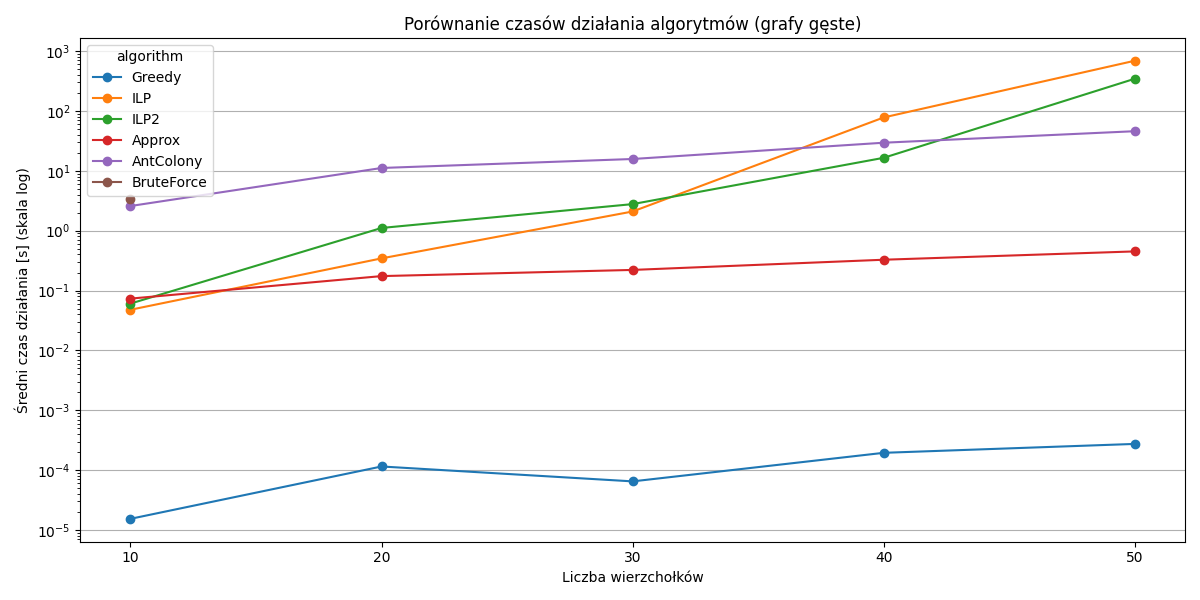
\includegraphics[width=\textwidth]{assets/dense.png}
        \caption{Porównanie średniego czasu działania algorytmów na grafach gęstych w stosunku do liczby wierzchołków w grafie.}
        \label{fig:densePlot}
    \end{figure}

    W tym przypadku znacznie wyróżnia się algorytm Greedy, który działa ponad 1000 razy szybciej niż pozostałe algorytmy, przy czym nie osiąga wyników znacznie odbiegających od optymalnego. Algorytm Approx jest również efektywny czasowo, mimo, że do jego konstrukcji użyto programowania liniowego. Najprawdopodobniej powodem takiego wyniku jest korzystna struktura grafu dla tego algorytmu.

    Naturalnie, wraz ze wzrostem liczby wierzchołków, a co za tym idzie i krawędzi, czas pracy wszystkich algorytmów wydłuża się. Dla algorytmu zachłannego są to jednak na tyle krótkie czasy, że można stwierdzić, że algorytm będzie skalowalny i również wykonywalny w rozsądnym czasie dla większych grafów.

    Algorytmy ILP i ILP2 notują mocny skok czasowy dla $n \geq 40 $. Jest on wyraźniejszy i większy niż dla grafów rzadkich, co jest spodziewanym zachowaniem, z racji większej liczby krawędzi do przeanalizowania. W tym przypadku udało się potwierdzić hipotezę, że algorytm ILP2 będzie szybszy od ILP, co ma miejsce dla większej liczby wierzchołków. Wynika to z dużej liczby cykli grafu gęstego do przeanalizowania przez algorytm ILP. ILP2, oparty na przepływach, działa znacznie szybciej. \\
    Algorytm mrówkowy w stosunku do pozostałych jest dosyć stabilny czasowo, jednakże jego jakość jest mierna.\\
    
    Gęste grafy posiadają dużo krawędzi, więc posiadają one wiele zbiorów dominujących. Algorytmy Approx i Greedy wykorzystują ochronę wielu wierzchołków z jednego wybranego, dlatego w tym przypadku wypadają one bardzo korzystnie czasowo i jakościowo. Ze względu na wzrost krawędzi, cierpią na tym algorytmy dokładne, ILP i ILP2. Heurystyka algorytmu mrówkowego jest nieefektywna dla tej klasy grafu.

    \begin{figure}[H]
        \centering
        \begin{subcaptionbox}*{}[0.48\linewidth]
            {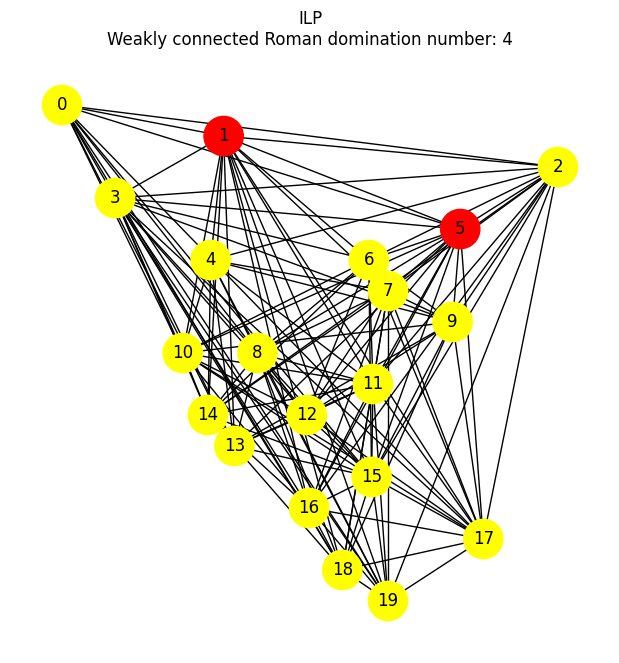
\includegraphics[width=0.75\linewidth]{assets/plots/ILP/ErdosRenyi_dense_n20_i2_results.png}}
        \end{subcaptionbox}
        \hfill
        \begin{subcaptionbox}*{}[0.48\linewidth]
            {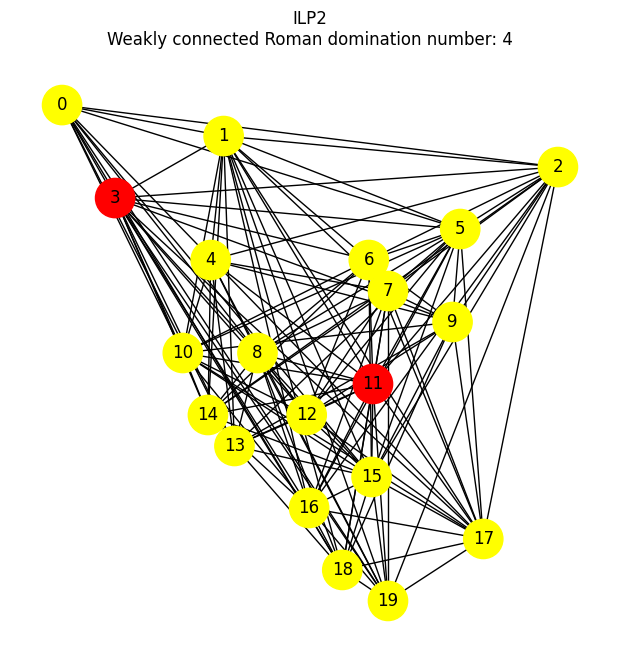
\includegraphics[width=0.75\linewidth]{assets/plots/ILP2/ErdosRenyi_dense_n20_i2_results.png}}
        \end{subcaptionbox}
        \hfill
        \begin{subcaptionbox}*{}[0.48\linewidth]
            {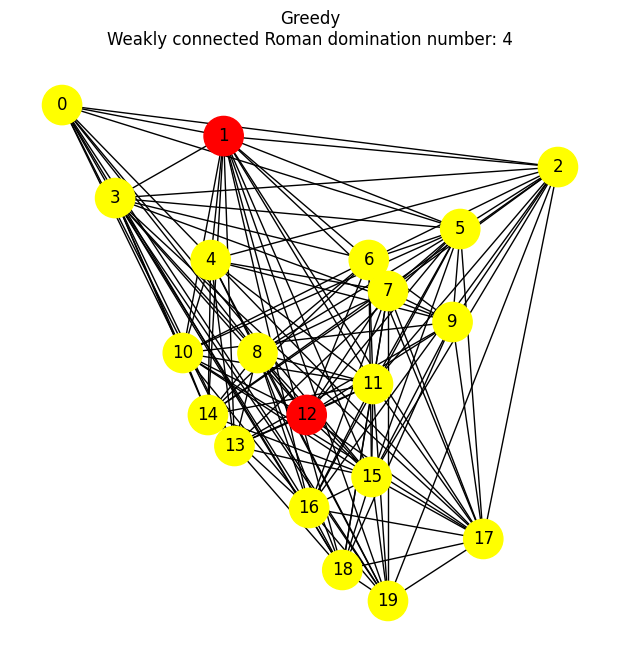
\includegraphics[width=0.75\linewidth]{assets/plots/Greedy/ErdosRenyi_dense_n20_i2_results.png}}
        \end{subcaptionbox}
        \hfill
        \begin{subcaptionbox}*{}[0.48\linewidth]
            {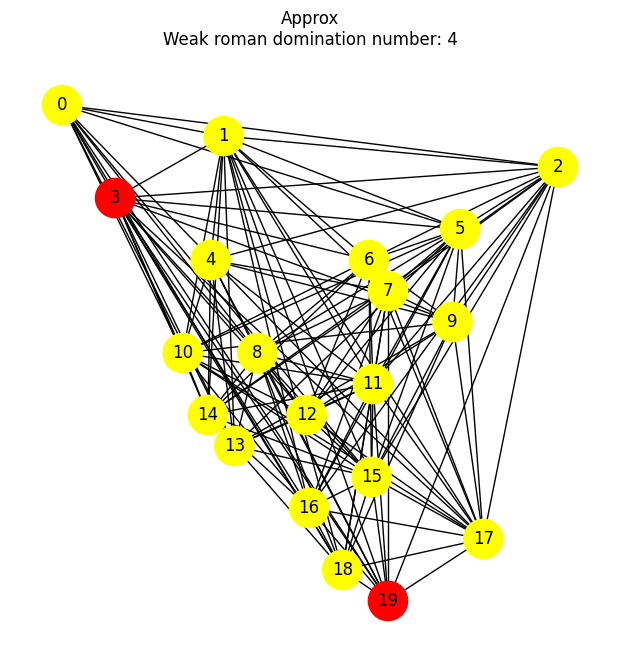
\includegraphics[width=0.75\linewidth]{assets/plots/Approx/ErdosRenyi_dense_n20_i2_results.png}}
        \end{subcaptionbox}
        \hfill
        \begin{subcaptionbox}*{}[0.48\linewidth]
            {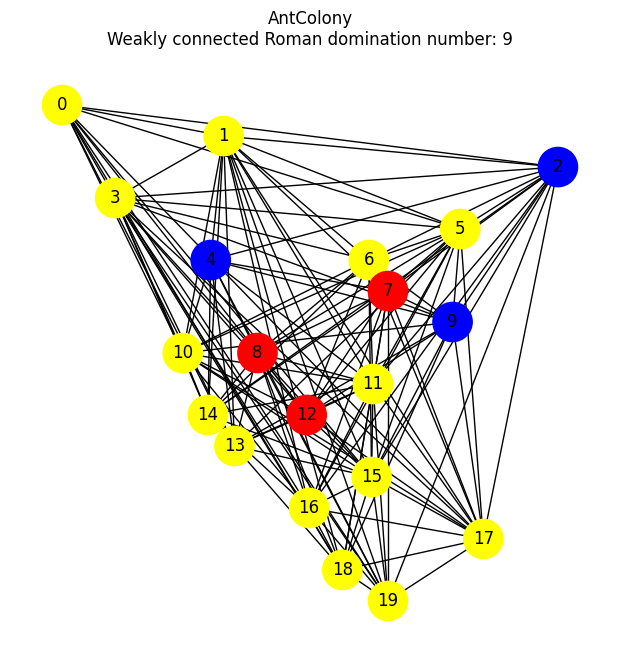
\includegraphics[width=0.75\linewidth]{assets/plots/AntColony/ErdosRenyi_dense_n20_i2_results.png}}
        \end{subcaptionbox}
    
        \caption{Wyniki dla przykładowego grafu gęstego.}
        \label{fig:dense}
    \end{figure}

\subsection{Drzewa}

Drzewa to grafy acykliczne, posiadające $n-1$ krawędzi dla $n$ wierzchołków. Są to grafy bardzo rzadkie, przez co ich zbiór dominujący jest bardzo często liczniejszy w stosunku do innych klas grafów o podobnym rozmiarze. Dlatego algorytmy deterministyczne i przybliżone, które nie są specjalnie dostosowane pod drzewa, mogą osiągać niezadowalające wyniki. Dla takiej uporządkowanej struktury za to można znaleźć efektywny algorytm specjalny tylko dla tej klasy grafu.

\begin{table}[H]
    \centering
    \begin{tabular}{|c|c|c|c|c|}
    \hline
    Algorytm & Liczba wierzchołków & Liczba krawędzi & $\gamma^{\text{wc}}_R(G)$ & Średni czas (s) \\
    \hline
    Greedy & 10 & 9 & 8 & 0,00005232 \\
    TreeLinear & 10 & 9 & 7 & 0,00051616 \\
    ILP & 10 & 9 & 7 & 0,04267752 \\
    ILP2 & 10 & 9 & 7 & 0,04535534 \\
    Approx & 10 & 9 & 14 & 0,3153601 \\
    Brute Force & 10 & 9 & 7 & 0,65010432 \\
    AntColony & 10 & 9 & 8 & 1,19096304 \\
    \hline
    Greedy & 20 & 19 & 12 & 0,00007772 \\
    TreeLinear & 20 & 19 & 12 & 0,00089554 \\
    ILP & 20 & 19 & 12 & 0,04966132 \\
    ILP2 & 20 & 19 & 12 & 0,07429058 \\
    Approx & 20 & 19 & 16 & 0,20606074 \\
    AntColony & 20 & 19 & 18 & 2,04032124 \\
    \hline
    Greedy & 30 & 29 & 20 & 0,0001205 \\
    TreeLinear & 30 & 29 & 17 & 0,00148292 \\
    ILP & 30 & 29 & 17 & 0,04517938 \\
    ILP2 & 30 & 29 & 17 & 0,13887008 \\
    Approx & 30 & 29 & 36 & 1,0127093 \\
    AntColony & 30 & 29 & 30 & 4,13727904 \\
     \hline
     Greedy & 40 & 39 & 33 & 0,00021536 \\
     TreeLinear & 40 & 39 & 29 & 0,0017755 \\
     ILP & 40 & 39 & 29 & 0,06708872 \\
     ILP2 & 40 & 39 & 29 & 0,48569172 \\
     Approx & 40 & 39 & 48 & 3,7790714 \\
     AntColony & 40 & 39 & 43 & 3,79114808 \\
    \hline
    Greedy & 50 & 49 & 45 & 0,00107456 \\
    TreeLinear & 50 & 49 & 35 & 0,00480282 \\
    ILP & 50 & 49 & 35 & 0,07759686 \\
    ILP2 & 50 & 49 & 35 & 0,82981668 \\
    Approx & 50 & 49 & 66 & 5,0276923 \\
    AntColony & 50 & 49 & 59 & 12,4118761 \\ 
    \hline
    \end{tabular}
    \caption{Wyniki dla drzew}
    \end{table}

    W tym przypadku algorytmy dokładnie wyznaczające $\gamma^{\text{wc}}_R(G)$ poradziły sobie również w rozsądnym czasie. Wynika to z bardzo rzadkiej struktury grafu. W pozostałych przypadkach, wraz ze wzrostem liczby wierzchołków wyniki osiągane przez algorytmy przybliżone były coraz gorsze jakościowo, co wynika ze specyficznej struktury grafu, gdzie wybór wierzchołków zbioru dominującego słabo spójnego jest nietypowy w stosunku do innych klas grafów. Godny odnotowania jest tutaj fakt, że akurat w tym przypadku algorytm mrówkowy poradził sobie lepiej niż Approx, ze względu na to, że Approx tworzy zbiór dominujący spójny z samymi wartościami 2, co dla drzew będzie wysoce nieoptymalne.

    \begin{figure}[H]
        \centering
        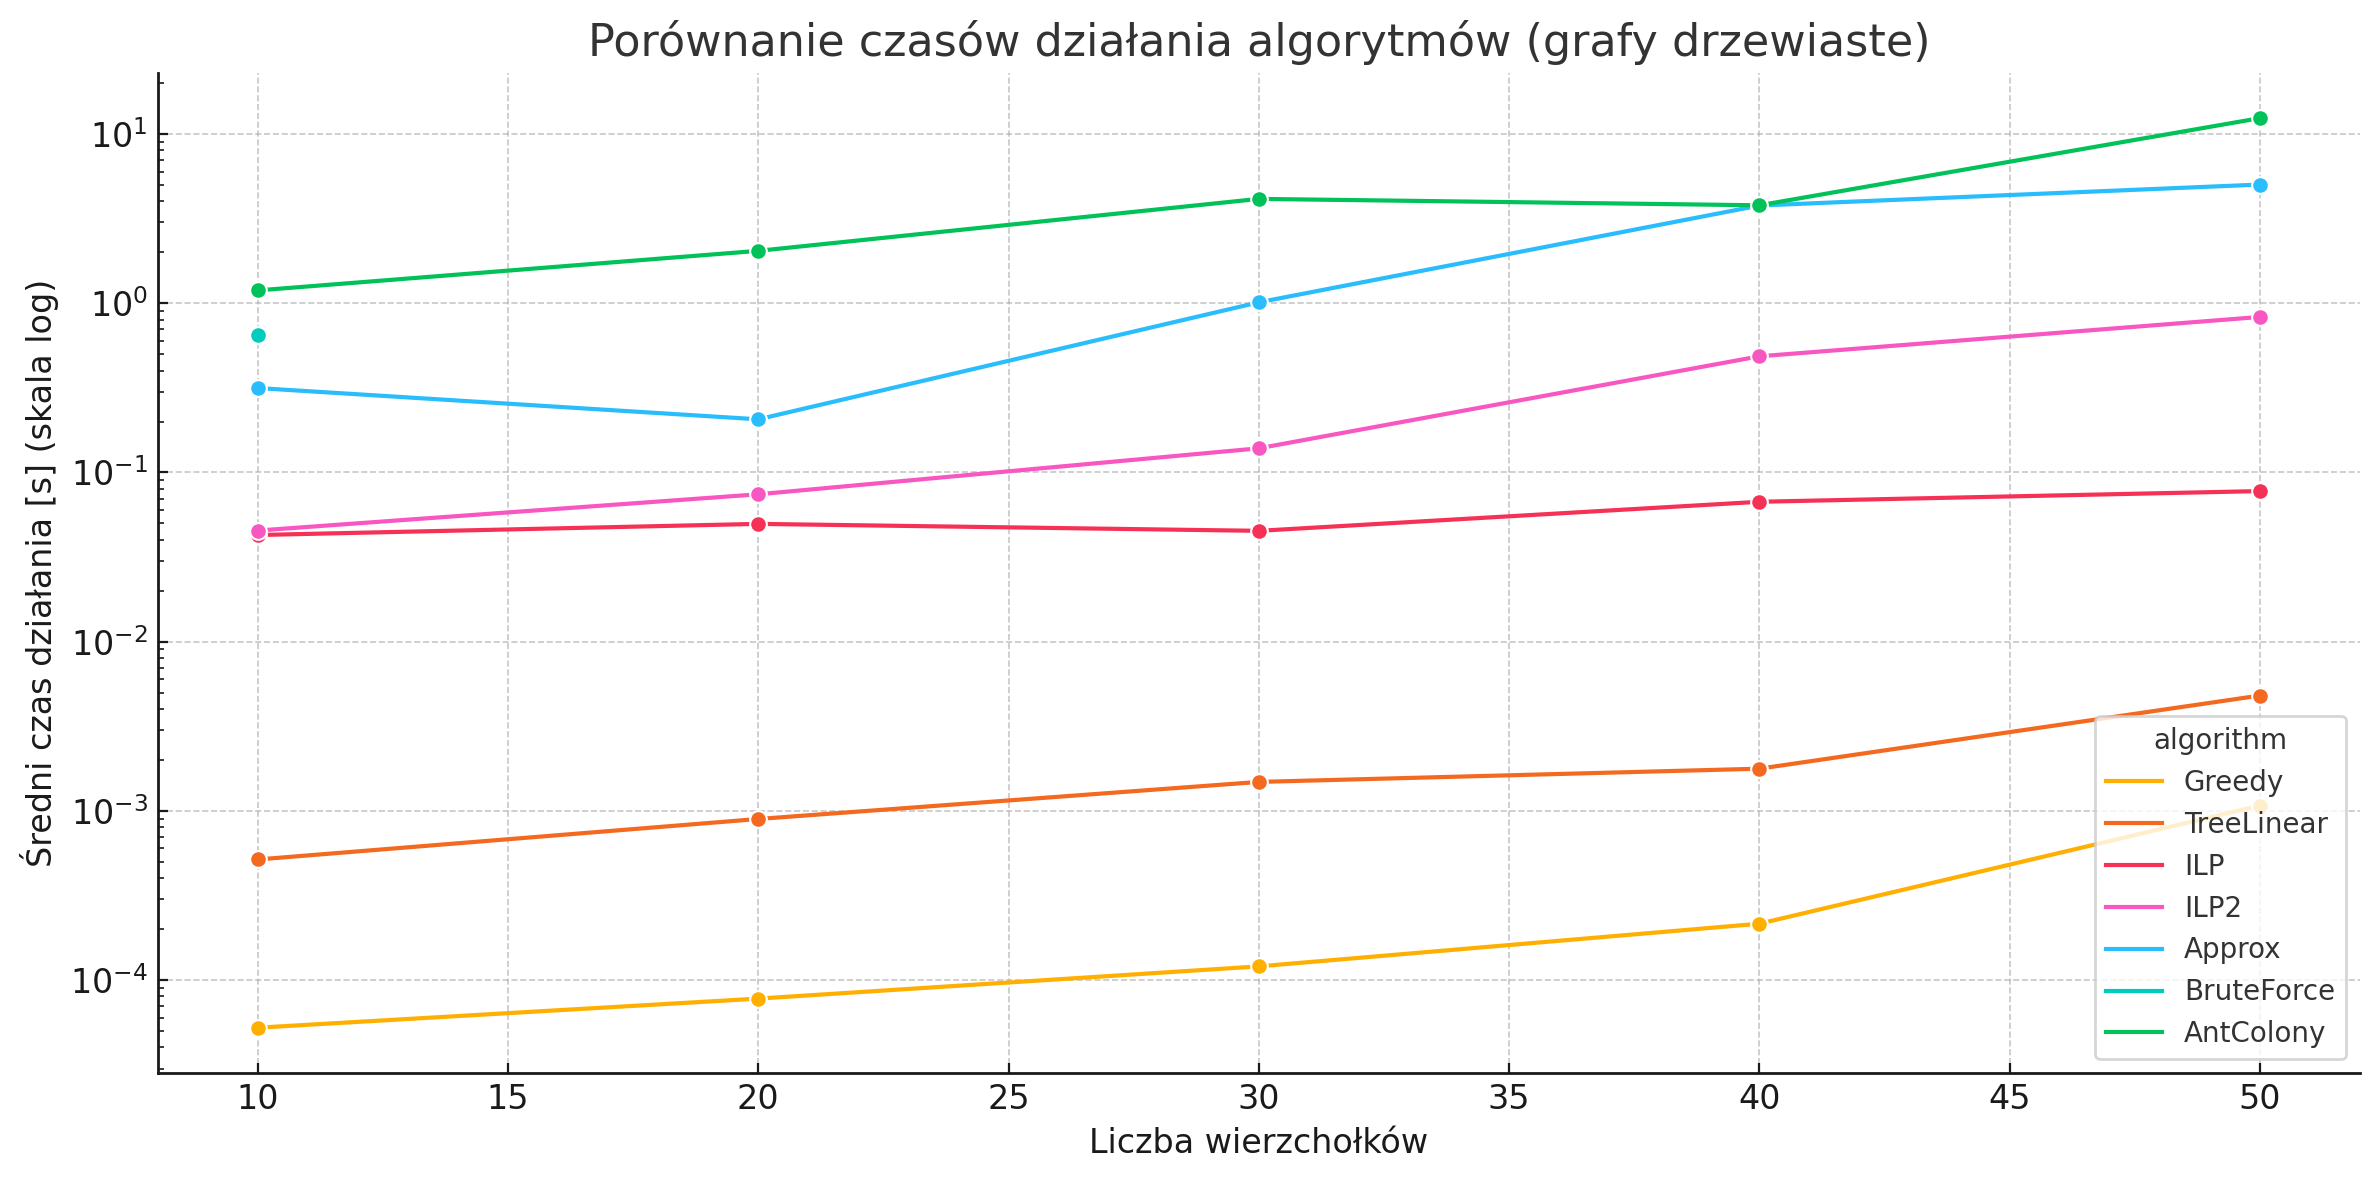
\includegraphics[width=\textwidth]{assets/trees.png}
        \caption{Porównanie średniego czasu działania algorytmów na drzewach w stosunku do liczby wierzchołków w grafie.}
        \label{fig:treePlot}
    \end{figure}

    Algorytm liniowy dla drzew daje w tym zestawieniu najlepszy stosunek czasu działania do jakości. Nie dość, że daje optymalny wynik, to dodatkowo w szybkim czasie. Algorytm jest skalowalny. Algorytmy ILP/ILP2 z powodu rzadkiej struktury grafu również wykonują się w rozsądnym czasie. ILP2 działa wolniej w tym przypadku od ILP. Zachłanny wykonuje się bardzo szybko, ale daje niekorzystne wyniki. TreeLinear jest tylko trochę wolniejszy, ale za to daje optymalny wynik. Algorytmy Approx oraz AntColony działają na tyle wolno i nieoptymalnie, że można stwierdzić, że nie nadają się dla drzew. Najlepszym wyborem dla tej klasy grafów jest algorytm liniowy dla drzew.

    \begin{figure}[H]
        \centering
        \begin{subcaptionbox}*{}[0.48\linewidth]
            {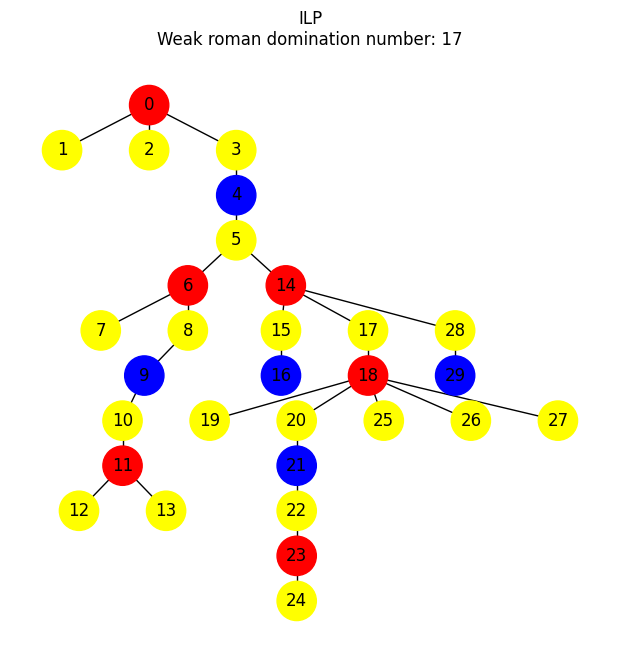
\includegraphics[width=0.75\linewidth]{assets/plots/ILP/RandomTree_n30_i2_results.png}}
        \end{subcaptionbox}
        \hfill
        \begin{subcaptionbox}*{}[0.48\linewidth]
            {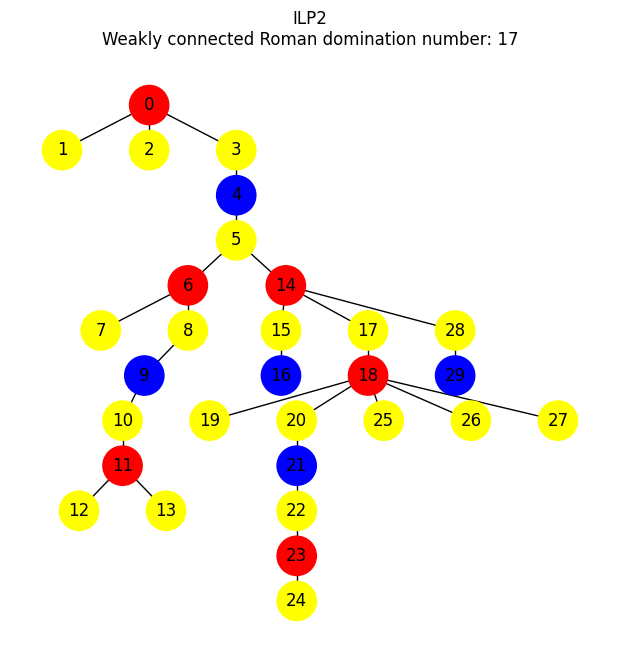
\includegraphics[width=0.75\linewidth]{assets/plots/ILP2/RandomTree_n30_i2_results.png}}
        \end{subcaptionbox}
        \hfill
        \begin{subcaptionbox}*{}[0.48\linewidth]
            {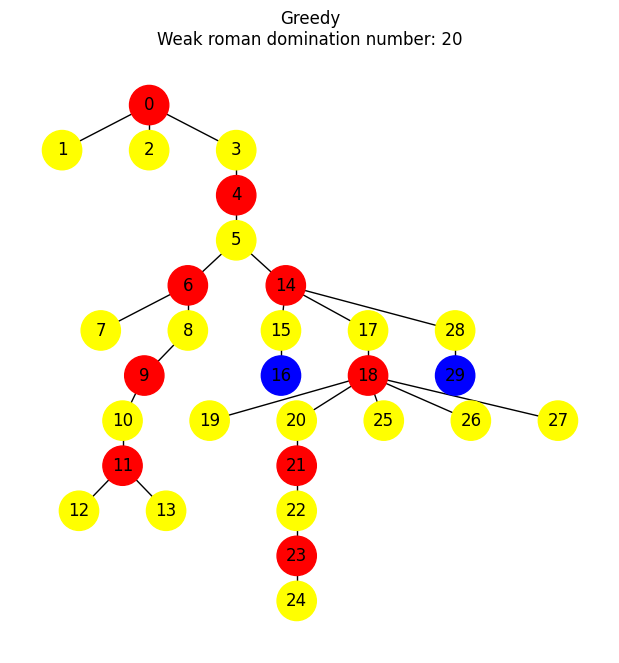
\includegraphics[width=0.75\linewidth]{assets/plots/Greedy/RandomTree_n30_i2_results.png}}
        \end{subcaptionbox}
        \hfill
        \begin{subcaptionbox}*{}[0.48\linewidth]
            {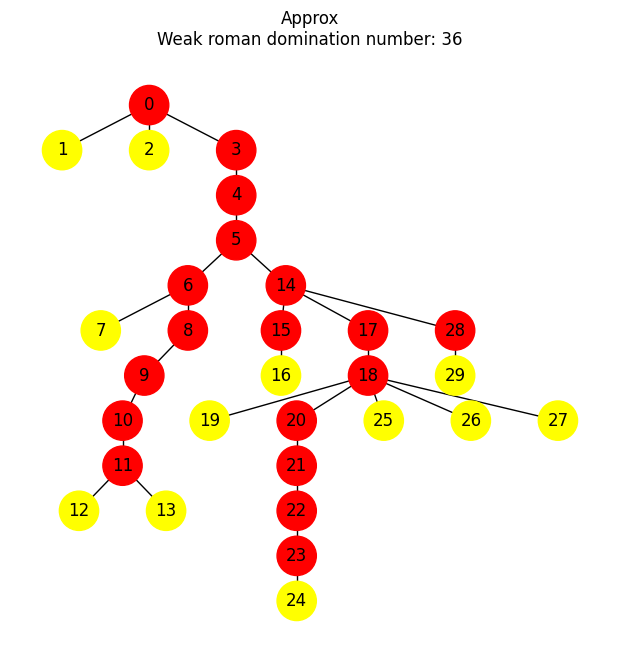
\includegraphics[width=0.75\linewidth]{assets/plots/Approx/RandomTree_n30_i2_results.png}}
        \end{subcaptionbox}
        \hfill
        \begin{subcaptionbox}*{}[0.48\linewidth]
            {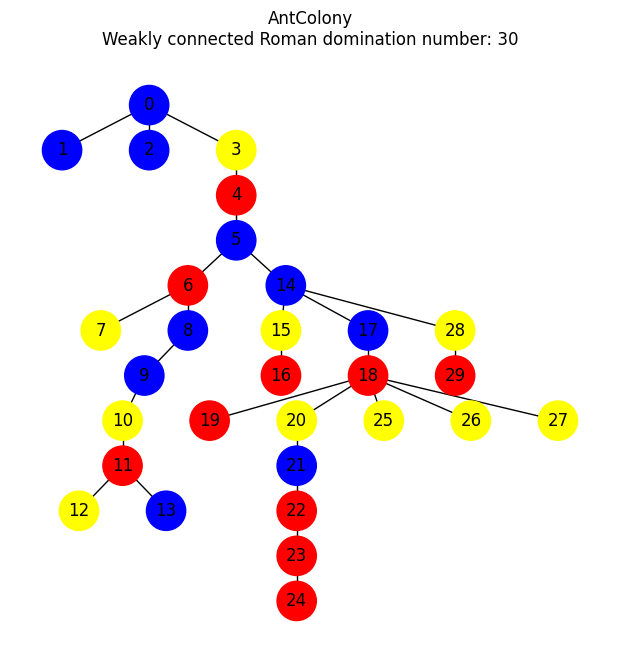
\includegraphics[width=0.75\linewidth]{assets/plots/AntColony/RandomTree_n30_i2_results.png}}
        \end{subcaptionbox}
        \hfill
        \begin{subcaptionbox}*{}[0.48\linewidth]
            {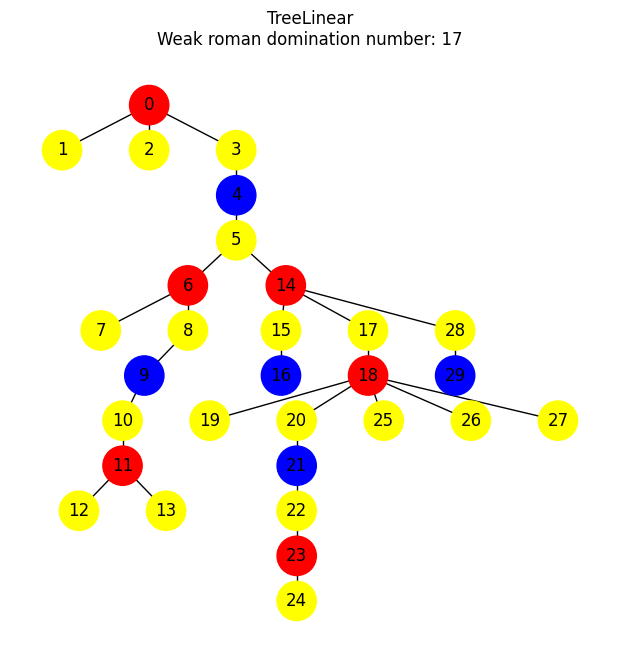
\includegraphics[width=0.75\linewidth]{assets/plots/TreeLinear/RandomTree_n30_i2_results.png}}
        \end{subcaptionbox}
    
        \caption{Wyniki dla przykładowego drzewa.}
        \label{fig:tree}
    \end{figure}


\subsection{Grafy bezskalowe}

Grafy bezskalowe to grafy naturalnie występujące w rzeczywistości, na przykład w biologii, sieciach WWW i społecznościowych, i są analizowane ze względu na potencjalne zastosowania praktyczne problemu WRCDF. Grafy te charakteryzują się wieloma wierzchołkami o małym stopniu i kilkoma wierzchołkami o dużym stopniu. Są to huby. Rozkład stopni wierzchołków w grafach tego typu jest potęgowy. Graf ten nie jest typowo gęsty, bo przeważają wierzchołki o niskim stopniu. Dlatego korzystne wyniki powinny osiągać algorytmy oparte na programowaniu liniowym.

\begin{table}[H]
    \centering
    \begin{tabular}{|c|c|c|c|c|}
    \hline
    Algorytm & Liczba wierzchołków & Liczba krawędzi & $\gamma^{\text{wc}}_R(G)$ & Średni czas (s) \\
    \hline
    Greedy & 10 & 25 & 2 & 0,00001166 \\
    ILP & 10 & 25 & 2 & 0,04384846 \\
    ILP2 & 10 & 25 & 2 & 0,05840188 \\
    Approx & 10 & 25 & 2 & 0,06902438 \\
    Brute Force & 10 & 25 & 2 & 2,3746041 \\
    AntColony & 10 & 25 & 3 & 3,02645522 \\
     \hline
     Greedy & 20 & 75 & 5 & 0,00008788 \\
     ILP & 20 & 75 & 4 & 0,1319412 \\
     Approx & 20 & 75 & 4 & 0,13767914 \\
     ILP2 & 20 & 75 & 4 & 0,25321824 \\
     AntColony & 20 & 75 & 9 & 8,82321618 \\ 
    \hline
    Greedy & 30 & 125 & 9 & 0,00009044 \\
    ILP & 30 & 125 & 6 & 0,08527778 \\
    ILP2 & 30 & 125 & 6 & 0,15141182 \\
    Approx & 30 & 125 & 6 & 0,16305526 \\
    AntColony & 30 & 125 & 18 & 10,0423744 \\ 
    \hline
    Greedy & 40 & 175 & 10 & 0,00026662 \\
    ILP & 40 & 175 & 7 & 0,1015079 \\
    Approx & 40 & 175 & 8 & 0,18101464 \\
    ILP2 & 40 & 175 & 7 & 0,3487031 \\
    AntColony & 40 & 175 & 24 & 9,48435894 \\
    \hline
    Greedy & 50 & 225 & 14 & 0,00024856 \\
    Approx & 50 & 225 & 10 & 0,17308662 \\
    ILP & 50 & 225 & 10 & 0,48920074 \\
    ILP2 & 50 & 225 & 10 & 0,82045656 \\
    AntColony & 50 & 225 & 35 & 20,21980648 \\
    
    \hline
    \end{tabular}
    \caption{Wyniki dla grafów bezskalowych}
    \end{table}

    Algorytmy ILP/ILP2/Approx zadowalająco pokrywają huby i w rozsądnym czasie, co w strukturze tego grafu jest bardzo ważne. Algorytm zachłanny jest niedokładny, ale wielkość błędu nie rośnie znacznie wraz ze wzrostem liczby wierzchołków. Algorytm mrówkowy nie dość, że za każdym razem działa najwolniej ze wszystkich propozycji, to daje wraz ze wzrostem liczby wierzchołków coraz gorsze wyniki. Po raz kolejny wskazuje to na brak doboru odpowiedniej heurystyki do tego problemu. Oczywiście algorytm Brute Force daje poprawny wynik, aczkolwiek jest on zupełnie nieskalowalny na większą liczbę wierzchołków niż kilkanaście.

    \begin{figure}[H]
        \centering
        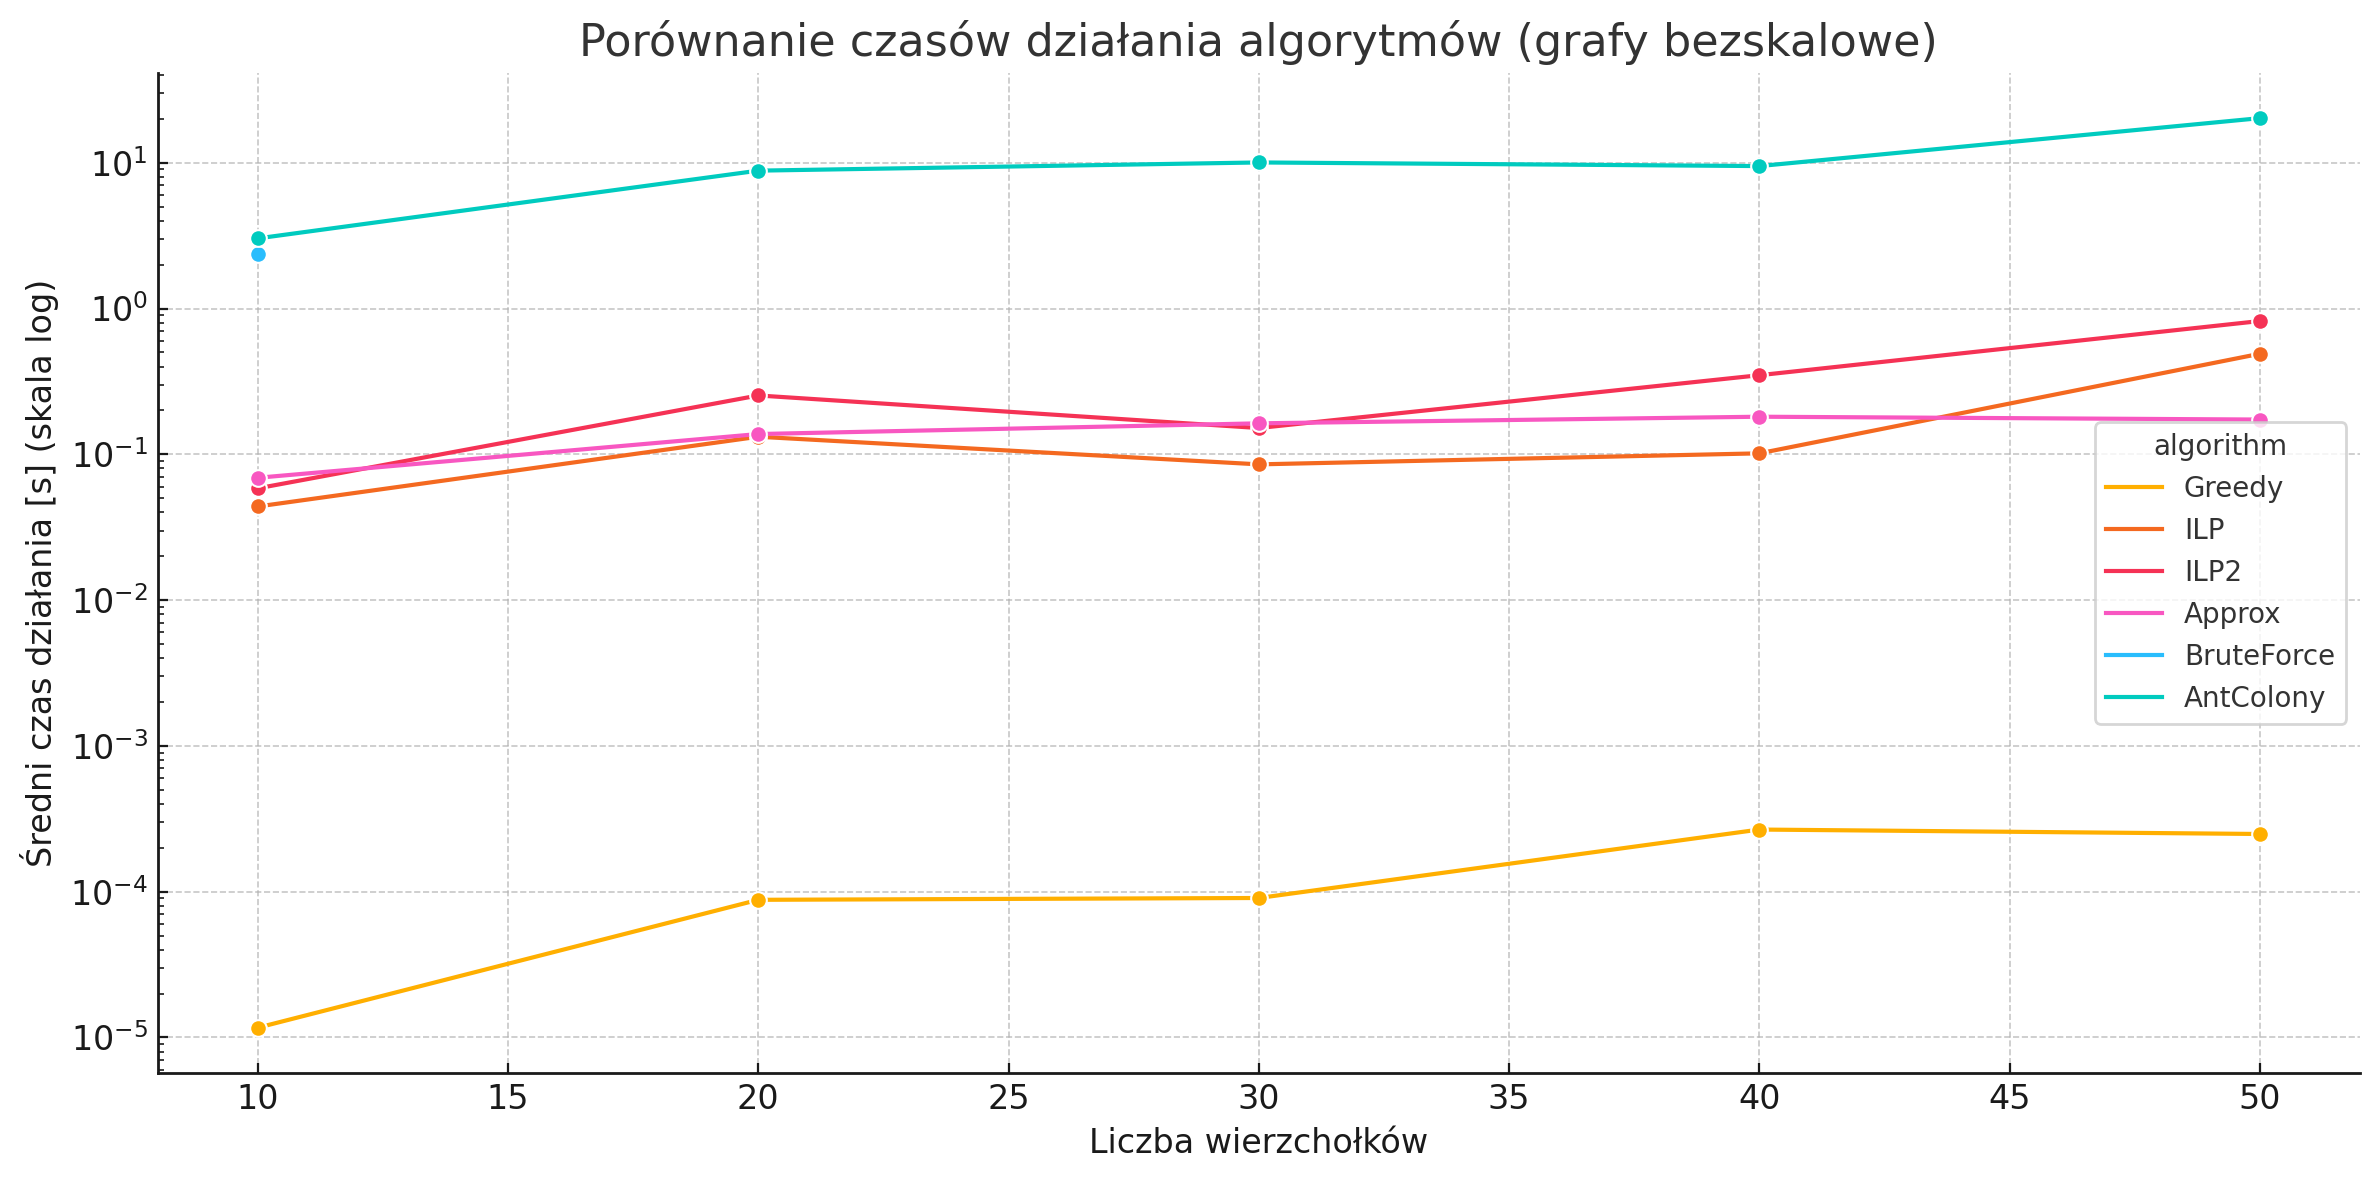
\includegraphics[width=\textwidth]{assets/scaleFree.png}
        \caption{Porównanie średniego czasu działania algorytmów na grafach bezskalowych w stosunku do liczby wierzchołków w grafie.}
        \label{fig:scaleFreePlot}
    \end{figure}

    Algorytmy Approx i Greedy są czasowo najefektywniejsze. Należy pamiętać, że Approx został zaimplementowany na podstawie programowania liniowego, więc wraz ze wzrostem liczby wierzchołków może zacząć działać bardzo długo. Algorytmy dokładne ILP/ILP2 działają w podobnym czasie co Approx. Algorytm mrówkowy jest przynajmniej 10 razy wolniejszy od innych algorytmów, co czyni go bardzo nieefektywnym.

    \begin{figure}[H]
        \centering
        \begin{subcaptionbox}*{}[0.48\linewidth]
            {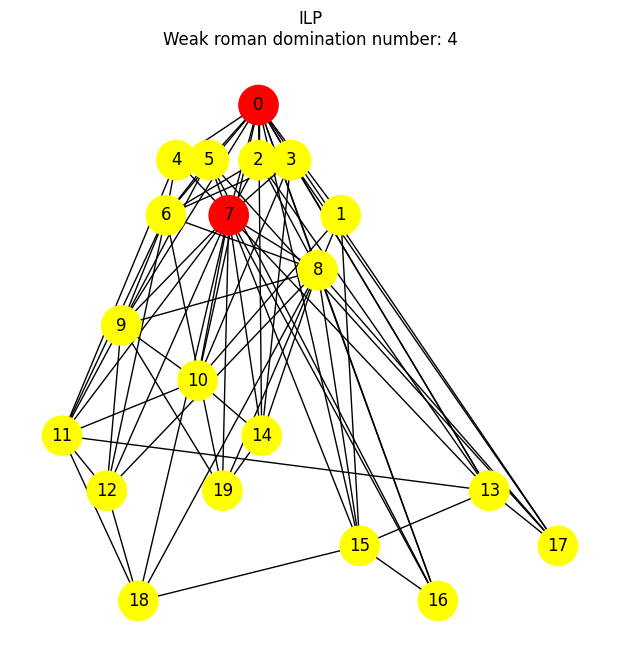
\includegraphics[width=0.75\linewidth]{assets/plots/ILP/ScaleFree_n20_i2_results.png}}
        \end{subcaptionbox}
        \hfill
        \begin{subcaptionbox}*{}[0.48\linewidth]
            {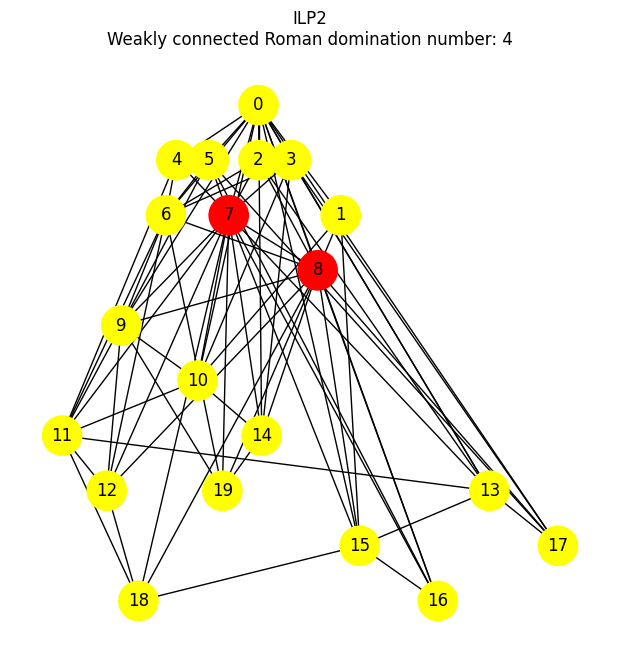
\includegraphics[width=0.75\linewidth]{assets/plots/ILP2/ScaleFree_n20_i2_results.png}}
        \end{subcaptionbox}
        \hfill
        \begin{subcaptionbox}*{}[0.48\linewidth]
            {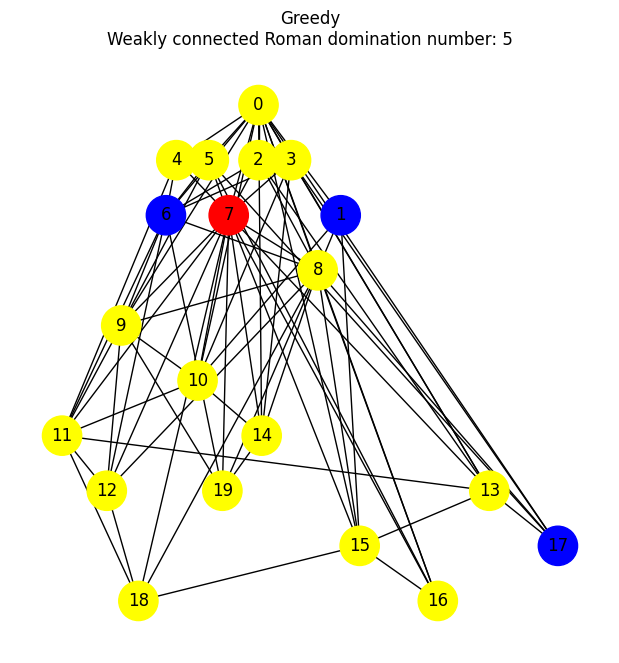
\includegraphics[width=0.75\linewidth]{assets/plots/Greedy/ScaleFree_n20_i2_results.png}}
        \end{subcaptionbox}
        \hfill
        \begin{subcaptionbox}*{}[0.48\linewidth]
            {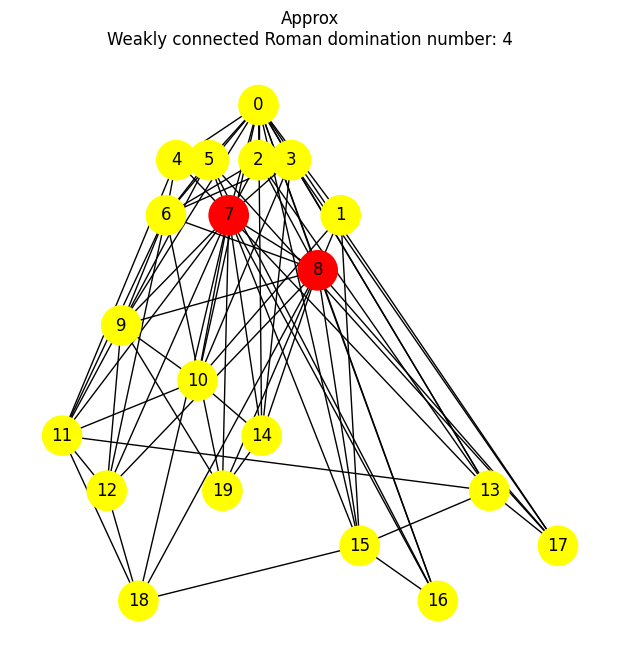
\includegraphics[width=0.75\linewidth]{assets/plots/Approx/ScaleFree_n20_i2_results.png}}
        \end{subcaptionbox}
        \hfill
        \begin{subcaptionbox}*{}[0.48\linewidth]
            {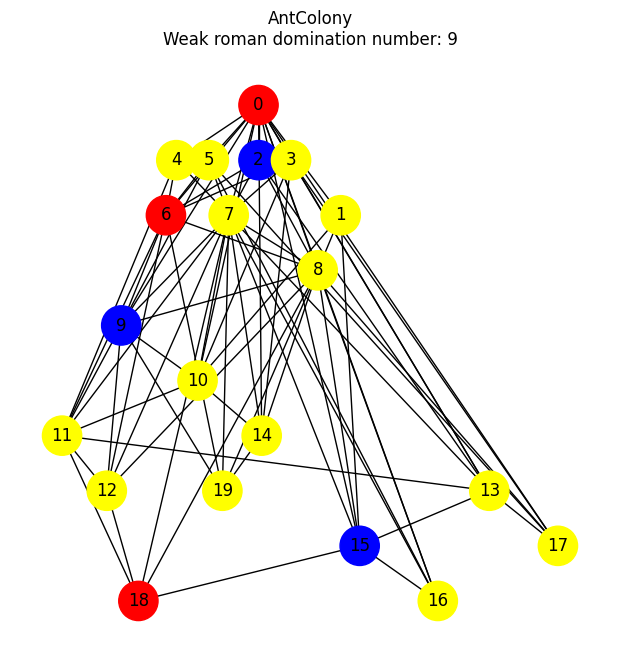
\includegraphics[width=0.75\linewidth]{assets/plots/AntColony/ScaleFree_n20_i2_results.png}}
        \end{subcaptionbox}
    
        \caption{Wyniki dla przykładowego grafu bezskalowego.}
        \label{fig:tree}
    \end{figure}

\section{Wyniki algorytmów niedokładnych}

\subsection{Algorytm mrówkowy}

\begin{figure}[H]
    \centering
    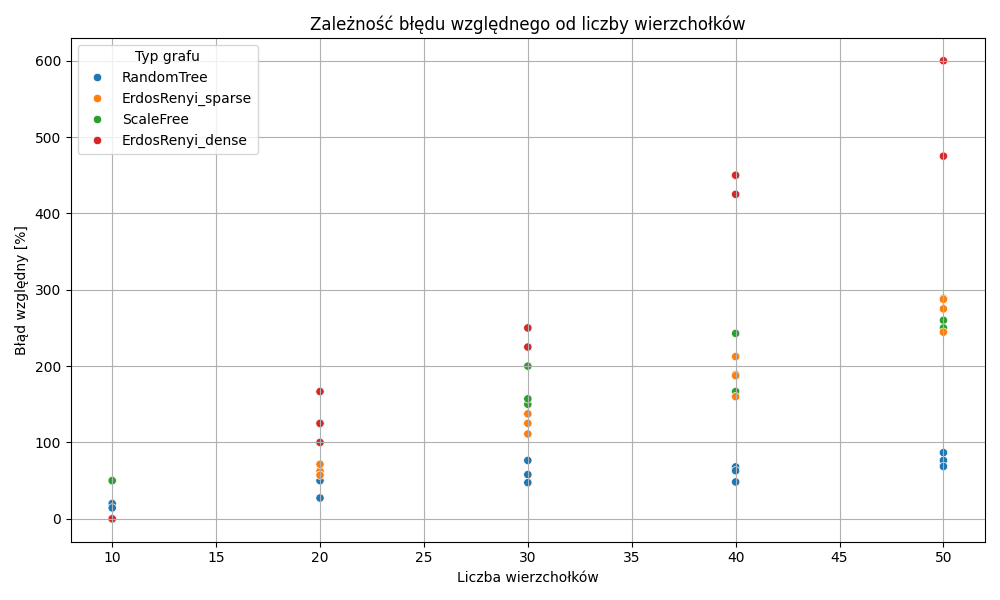
\includegraphics[width=\textwidth]{assets/plots_approx/ants.png}
    \caption{Zależność błędu względnego algorytmu mrówkowego od liczby wierzchołków.}
    \label{fig:antsPlot}
\end{figure}

Wraz ze wzrostem liczby wierzchołków można zaobserwować coraz większą rozbieżność od najmniejszej $\gamma^{\text{wc}}_R(G)$. Dla mniejszych grafów prościej trafić na rozwiązanie optymalne, niż eksplorowanie całej przestrzeni rozwiązań w większych grafach.

Największą rozbieżność można zaobserwować dla grafów gęstych, gdzie błąd względny osiąga nawet 600\%. Wynika to z tego, że w grafach gęstych jest dużo wierzchołków o wysokich stopniach, więc heurystyka oparta na stopniach wierzchołków nie jest w stanie wyróżnić wierzchołków najbardziej nadających się do zbioru dominującego.

W odróżnieniu do grafów gęstych, algorytm osiągał zadowalające wyniki dla drzew. Wynika to z tego, że drzewa są grafami rzadkimi i nie ma tam wielu połączeń wierzchołkowych do analizy. W odróżnieniu do innych klas grafów, struktura drzew sprzyja lokalnym decyzjom dotyczącym dominowania, dlatego też algorytm mrówkowy radzi sobie nienajgorzej, chociaż wciąż mocno odbiega od optymalnego wyniku.\\
Pośrednie wyniki osiągają grafy rzadkie i bezskalowe.

\subsection{Algorytm zachłanny}

\begin{figure}[H]
    \centering
    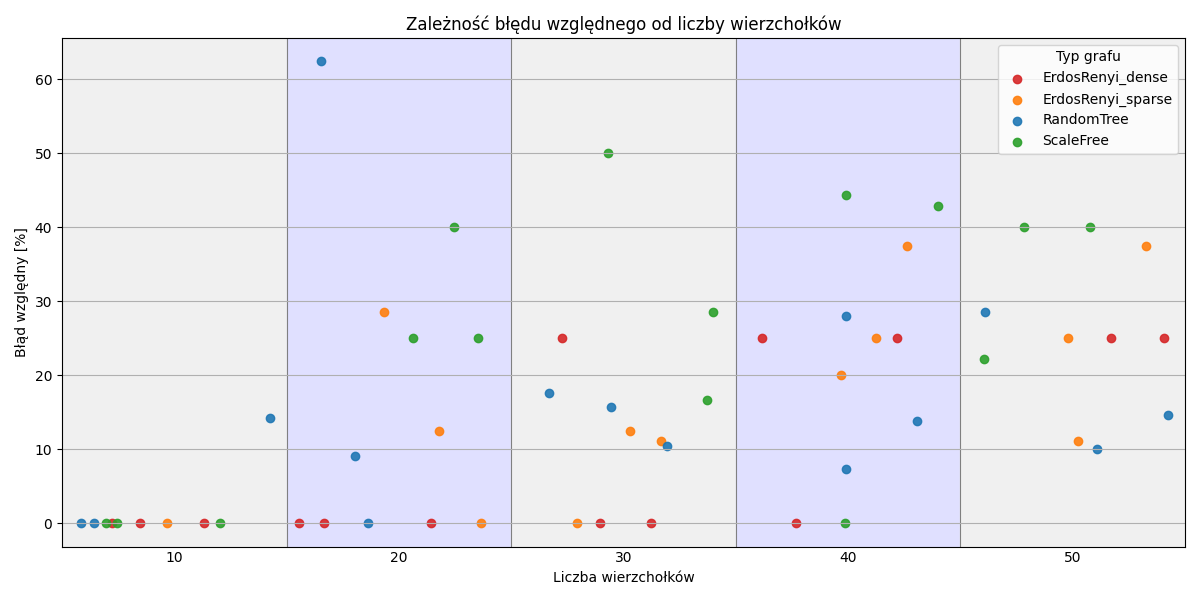
\includegraphics[width=\textwidth]{assets/plots_approx/greedy.png}
    \caption{Zależność błędu względnego algorytmu zachłannego od liczby wierzchołków.}
    \label{fig:greedyPlot}
\end{figure}

Algorytm zachłanny charakteryzuje się ogólnie niskim błędem względnym na tle innych prezentowanych algorytmów. Godny odnotowania jest fakt, że wraz ze wzrostem liczby wierzchołków w grafach, algorytm nie traci znacznie na jakości, dlatego na podstawie tych przykładu można wysnuć hipotezę, że algorytm może być jakościowo skalowalny.

Największy średni błąd względny algorytm osiąga dla grafów rzadkich i bezskalowych. Prawdopodobnym powodem tego są nieregularne struktury tych grafów i konieczność nieoczywistych decyzji odnośnie wyboru wierzchołka należącego do zbioru dominującego słabo spójnego.

Algorytm zachłanny wyjątkowo dobrze radzi sobie z grafami gęstymi. Wynika to z tego, że promowane są wierzchołki, które pokrywają jak najwięcej sąsiadów. Dla grafów gęstych strategia ta jest bardzo korzystna i sprawia, że algorytm jest w stanie osiągnąć wynik optymalny, bądź bardzo bliski optymalnemu.

Z racji tego, że algorytm zachłanny tworzy dominowanie bardziej lokalnie, od wierzchołka o największym stopniu, bez zwrócenia uwagi na całą strukturę grafu, to w zależności od konkretnego przypadku testowego drzewa, wyniki mogą być bardzo dobre, bądź wysoce nieoptymalne. Na prezentowanym wykresie przypadek, największego błędu względnego: ponad 60\%, zaobserwowano właśnie dla drzewa.  

\subsection{Algorytm aproksymacyjny}

\begin{figure}[H]
    \centering
    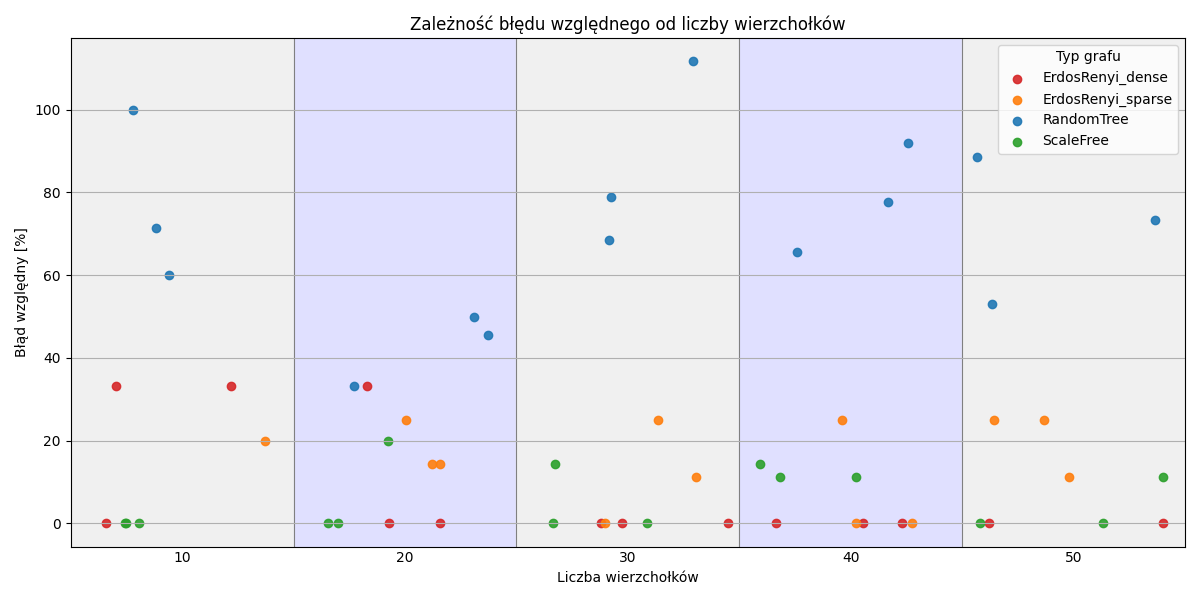
\includegraphics[width=\textwidth]{assets/plots_approx/approx.png}
    \caption{Zależność błędu względnego algorytmu aproksymacyjnego od liczby wierzchołków.}
    \label{fig:approxPlot}
\end{figure}

Dla grafów gęstych algorytm Approx osiąga bardzo dobre wyniki, w wielu przypadkach optymalne, ze względu na dużą liczbę małych zbiorów dominujących.

Z kolei dla drzew jest to bardzo zła strategia. Algorytm przez to, że wyznacza CDS i przypisuje wszystkim wierzchołkom CDS wartości 2, sprawia, że istnieje bardzo dużo nadmiernych przypisań, przez co dla drzew algorytm potrafi osiągnąć nawet ponad 100\% błędu względnego.

Algorytm aproksymacyjny radzi sobie dobrze z grafami rzadkimi i bezskalowymi, z błędem względnym na poziomie 20-40\%. Wyznacza on prawidłowo CDS i dla tych klas grafów najwyraźniej wystarcza to dla osiągnięcia niskiego poziomu błędu względnego.\\

Wykres przedstawia porównanie rzeczywistego współczynnika aproksymacji algorytmu Approx z jego teoretyczną granicą ustaloną w artykule \cite{ILP} wynoszącą $2(1+\epsilon)(1 + \ln(\Delta - 1))$ w zależności od maksymalnego stopnia wierzchołka w grafie.

\begin{figure}[H]
    \centering
    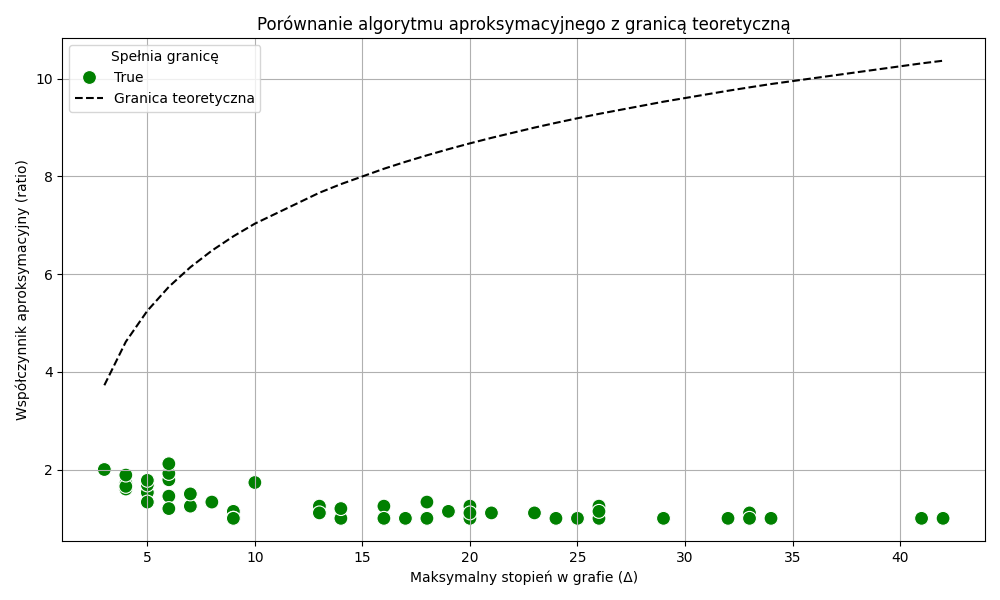
\includegraphics[width=\textwidth]{assets/plots_approx/image.png}
    \caption{Porównanie algorytmu aproksymacyjnego z granicą teoretyczną $2(1+\epsilon)(1 + \ln(\Delta - 1))$.}
    \label{fig:approxPlot}
\end{figure}

Można zauważyć, że wszystkie wygenerowane przypadki testowe mieszczą się w granicy teoretycznej błędu. Granica teoretyczna znajduje się daleko od wygenerowanych przykładowych grafów. Zatem w praktyce algorytm radzi sobie znacznie lepiej niż granica teoretyczna zakłada. Prawdopodobnie istnieją przypadki znajdujące się blisko tej granicy, ale taki przypadek nie został odnaleziony w procesie testowania. Dlatego można potwierdzić fakt, że algorytm jest zgodny z współczynnikiem aproksymacji i nie przekracza przewidzianego maksimum, a przynajmniej nie znaleziono przypadku, żeby tak nie było. Można też zauważyć, że wraz ze wzrostem maksymalnego stopnia wierzchołka w testowym grafie, współczynnik aproksymacyjny algorytmu jest coraz niższy. Można z tego wywnioskować fakt, że algorytm jest w stanie dobrze wykorzystać obecność wierzchołków o wysokim stopniu, gdyż bardzo często są one częścią zbioru dominującego.

\subsection{Porównanie algorytmów przybliżonych}

\begin{figure}[H]
    \centering
    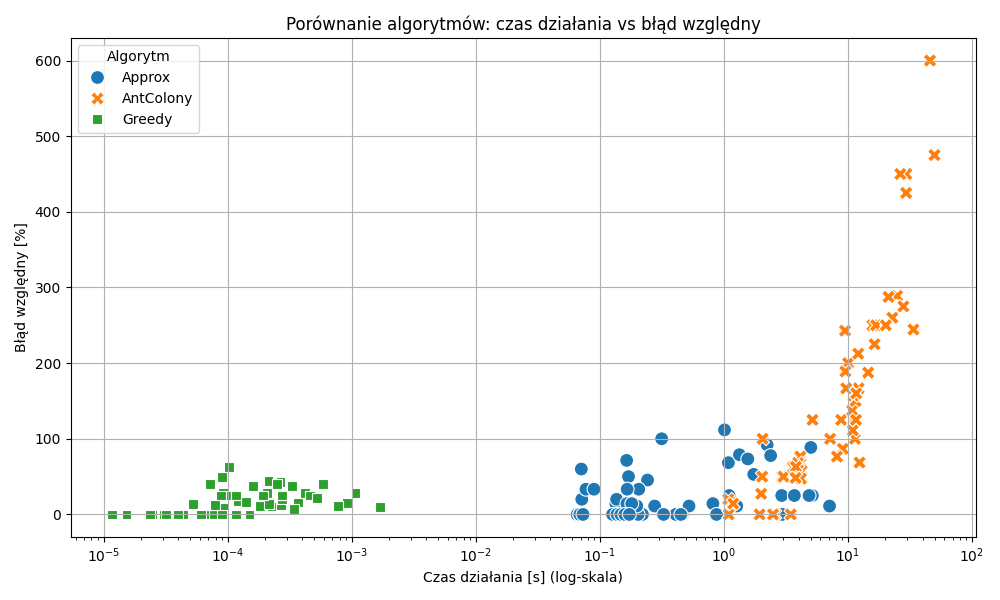
\includegraphics[width=\textwidth]{assets/plots_approx/alorithms.png}
    \caption{Algorytmy przybliżone: czas działania w stosunku do błędu względnego.}
    \label{fig:approxPlot}
\end{figure}

W ujęciu porównawczym wszystkich algorytmów wyznaczających $\gamma^{\text{wc}}_R(G)$ w sposób przybliżony, algorytm zachłanny prezentuje najlepszy stosunek czasu działania do jakości rozwiązania. Jego rozwiązanie, dla wygenerowanych przepadków testowych można otrzymać w przedziale $10^{-5}$ do $10^{-3}$ sekund, a błąd względny utrzymuje się na poziomie 0\%-50\%.\\
Algorytm Approx prezentuje czas działania w przedziale kilku sekund, potrafi znaleźć więcej lepszych rozwiązań niż Greedy, o czym świadczy większe zagęszczenie niebieskich punktów na poziomie ,,0'' niż w przypadku Greedy. Jednak czasem, zwłaszcza dla drzew, algorytm ten daje nieoptymalne wyniki.\\
Algorytm mrówkowy, w porównaniu z resztą radzi sobie najgorzej. Czas działania jest najdłuższy, bo rzędu od kilku do kilkudziesięciu sekund, dając przy tym znacznie gorsze wyniki, z największymi błędami względnymi. Świadczy to o tym, że w obecnej konfiguracji i dobranej heurystyce, algorytm mrówkowy nie radzi sobie z tym problemem.